\documentclass[letter,graphicx]{beamer}



\mode<presentation>
{
  \usetheme{Warsaw}
  % or ...

  \setbeamercovered{transparent}
  % or whatever (possibly just delete it)
}


\usepackage[english]{babel}
% or whatever

\usepackage[latin1]{inputenc}
% or whatever
\usepackage{verbatim}
\usepackage{times}
\usepackage[T1]{fontenc}
\usepackage{mychicago}
\renewcommand{\citeN}{\shortciteN}
% Or whatever. Note that the encoding and the font should match. If T1
% does not look nice, try deleting the line with the fontenc.

%\logo{
\includegraphics[width=.1\textwidth]{./images/official_NOAA_logo.pdf}}
\logo{}

\title[microhaplotypes from NGS] % (optional, use only with long paper titles)
{Reaching haplotopia: the promise and practice \\
of short-read microhaplotypes\\
in molecular ecology}

\subtitle{} % (optional)

\author[Eric C. Anderson] % (optional, use only with lots of authors)
{Eric C.~Anderson}
% - Use the \inst{?} command only if the authors have different
%   affiliation.

\institute[NOAA Fisheries] % (optional, but mostly needed)
{\mbox{}
%Fisheries Ecology Division \\ Southwest Fisheries Science Center \\ Santa Cruz, CA \\ USA
\hfill
\includegraphics[height=.25\textwidth]{./mhap_figs/juvie_rockfish.png}
\hfill
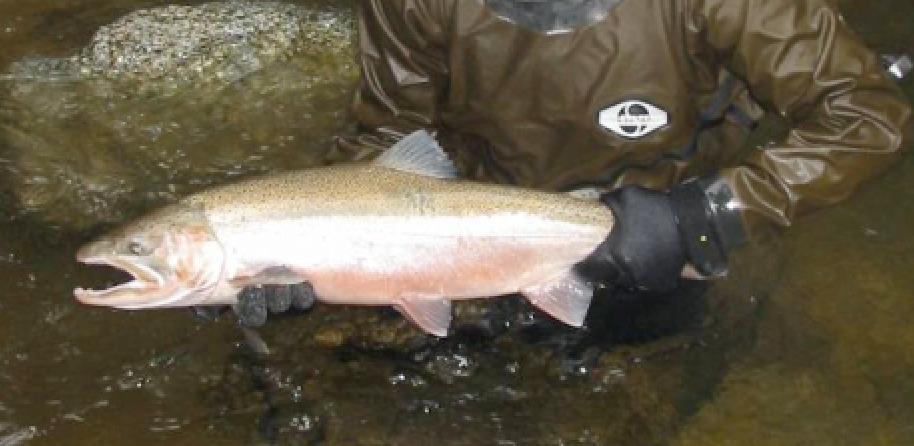
\includegraphics[height=.25\textwidth]{./mhap_figs/steelhead.png}
\hfill\mbox{}
}
% - Use the \inst command only if there are several affiliations.
% - Keep it simple, no one is interested in your street address.

\date[ConGen 2018] % (optional)
{
Conservation Genomics Workshop\\ 11 SEP 2018}

\subject{Talks}


%% More eric commands for inserting some small figures
\newcommand{\smikid}{\includegraphics[width=3.7ex]{images/smiley_blue_kid.pdf}}
\newcommand{\smired}{\includegraphics[width=2.9ex]{images/smiley_sad_red.png}}
\newcommand{\smiblue}{\includegraphics[width=2.9ex]{images/smiley_happy_blue.png}}
\newcommand{\thh}{^\mathrm{th}}
\newcommand{\tc}{\textcolor}
\def\bm#1{\mathpalette\bmstyle{#1}}
\def\bmstyle#1#2{\mbox{\boldmath$#1#2$}}


\begin{document}




\begin{frame}
  \titlepage
\end{frame}



\begin{frame}{Collaborators and Acknowledgments}
\begin{columns}
\begin{column}{0.6\textwidth}
NOAA/SWFSC/UCSC
\begin{itemize}
\item Carlos Garza
\item Anthony Clemento
\item Thomas Ng (UCSC grad student)
\item Diana Baetscher (UCSC grad student)
\end{itemize}
\end{column}


\begin{column}{0.4\textwidth}
UCSC Rockfish Project:
\begin{itemize}
\item Mark Carr
\item Chris Edwards
\item Dan Malone
\item Emily Saarman
\item Patrick Drake
\item Anna Lowe 
\end{itemize}
{\centering 

\includegraphics[width=0.7\textwidth]{mhap_figs/nsf.jpg}
}
\end{column}
\end{columns}
\end{frame}

%	Chris Edwards <cedwards@ucsc.edu>,
%Mark Carr <mhcarr@ucsc.edu>,
%John Carlos Garza <carlos.garza@noaa.gov>,
%"Eric C. Anderson" <eric.anderson@noaa.gov>,
%Emily Saarman <esaarman@ucsc.edu>,
%Daniel Malone <dmalone@ucsc.edu>,
%Patrick Drake <pdrake@ucsc.edu>,
%Anna Lowe <ablowe@ucsc.edu>
% Thomas Ng
% Diana Baetscher
%



\begin{frame}{Overview}
\begin{enumerate}
\item Larval dispersal and genetic patterns
\item Kelp-rockfish recruitment project
\item Next-generation sequencing and microhaplotypes
\item Confirmation of our data quality
\item Preliminary relationship inference work
\end{enumerate}

\end{frame}







\begin{frame}{Larval dispersal patterns influence many things}

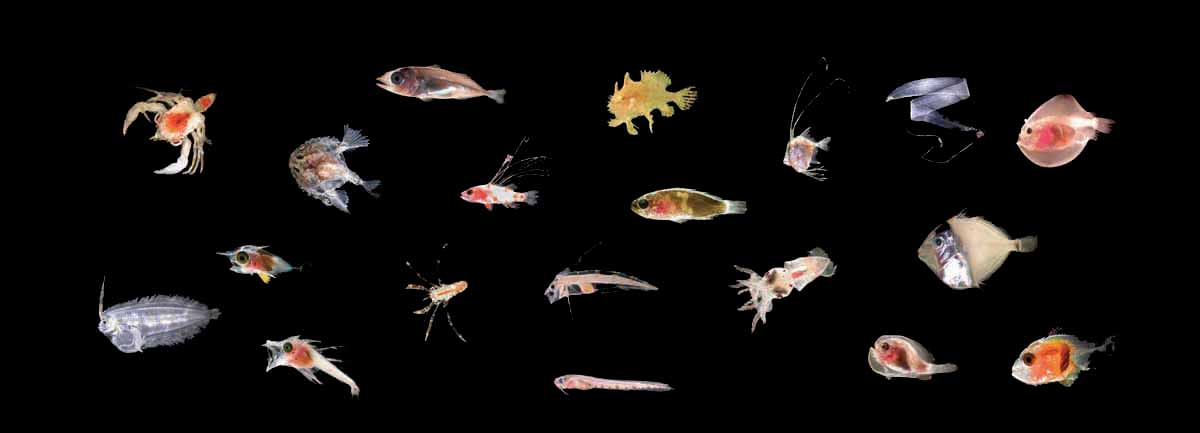
\includegraphics[width = \textwidth]{./figs/many_larvae.jpg}\\
{\tiny \vspace*{-4.5ex} \textcolor{white}{~rsmas.miami.edu}}

{\small
\begin{itemize}
\item Dynamics of recruitment and populations
\item The effects of fishing
\item The utility of different MPA designs
\item \ldots and it is just fascinating from a behavioral ecology perspective
\end{itemize}
}
\end{frame}




\begin{frame}{Try to study larval dispersal by linking larvae to parents}
\framesubtitle{``Integrative evaluation of larval dispersal and delivery in kelp rockfish using {\em inter-generational genetic tagging}, demography and
oceanography''}
{\small Mark Carr (PI), Chris Edwards, Carlos Garza, Eric Anderson (Co-PIs)}\\
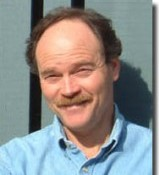
\includegraphics[height=.2\textheight]{./figs/mcarr.jpg}
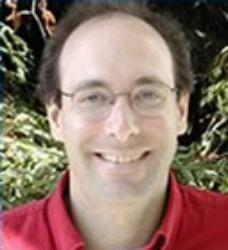
\includegraphics[height=.2\textheight]{./figs/cedwards.jpg}
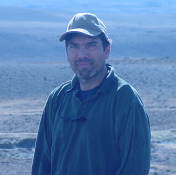
\includegraphics[height=.2\textheight]{./figs/carlos.png} \\

$\bullet$ {\bf Goal:} use parentage inference to accurately estimate the degree of self-recruitment of kelp rockfish in Carmel Bay, and integrate this with fine-scale current modeling.

$\bullet$ I will be talking about the genetic tools we have developed to do this.
\end{frame}





\begin{frame}{Kelp rockfish ({\em Sebastes atrovirens})}
\begin{center}
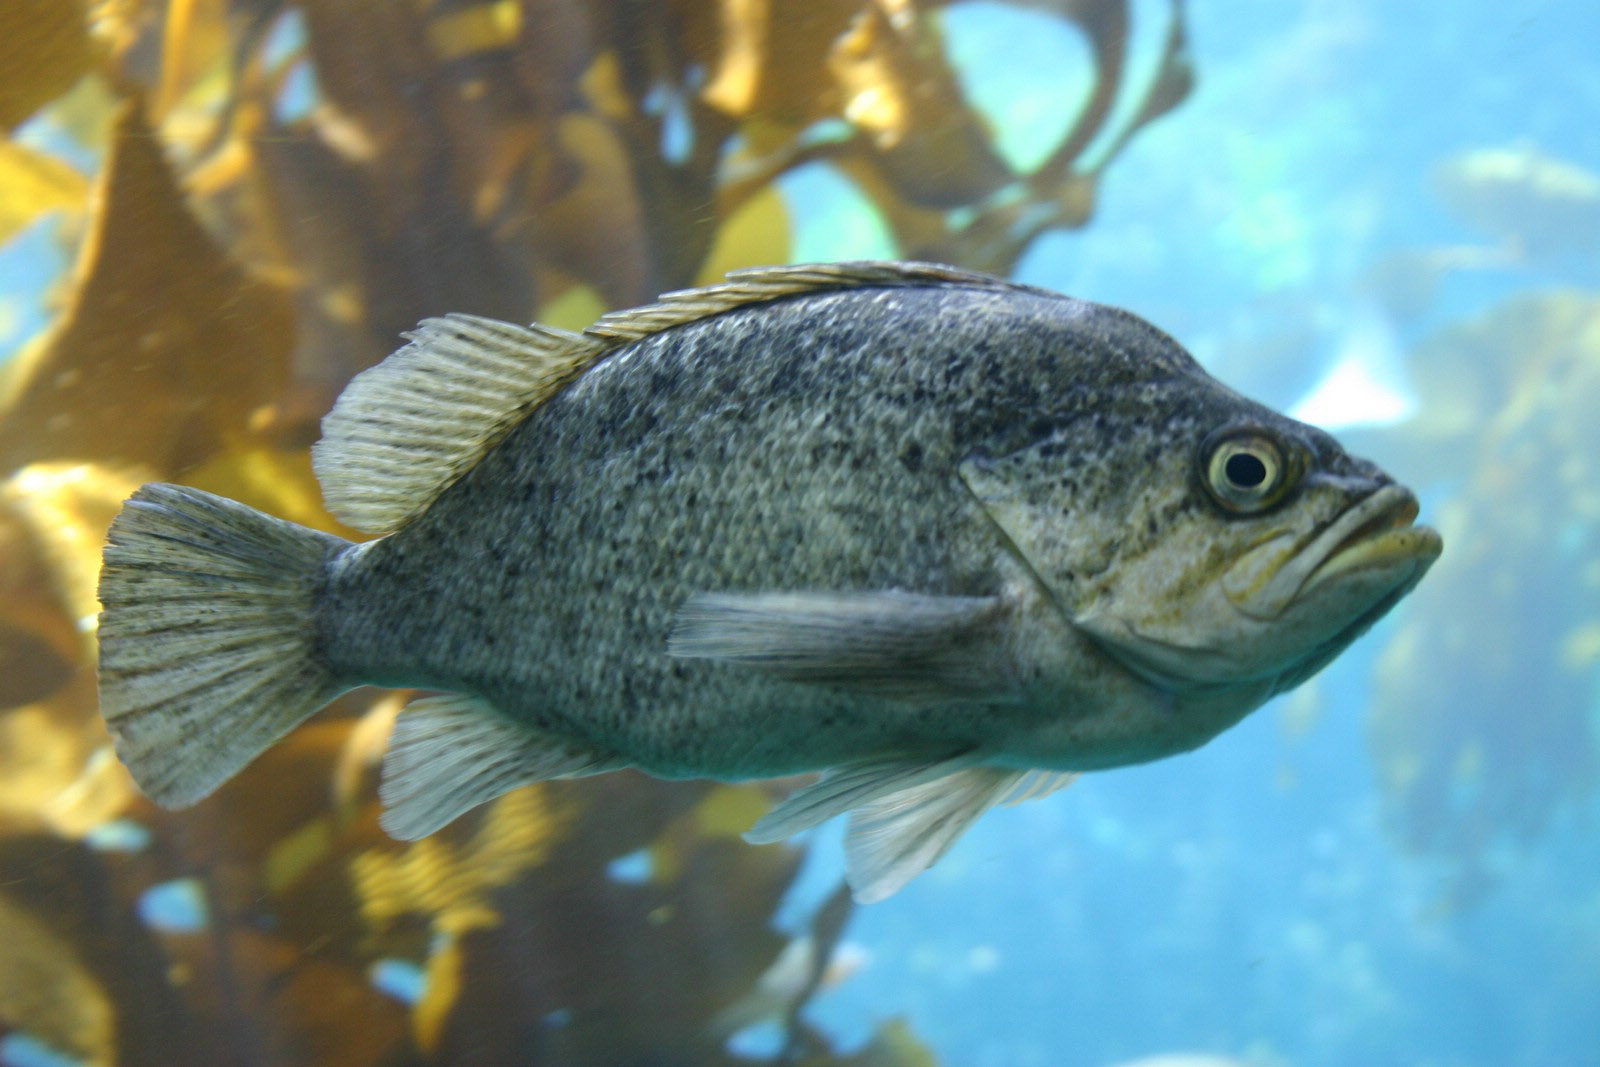
\includegraphics[width=.7\textwidth]{./figs/kelpy.jpg}\\
{\tiny \vspace*{-6ex} \textcolor{white}{photo: Chad King}}
\end{center}
{\tiny  Strongly associated with {\em Macrocystis}; $\approx$ Santa Cruz to Baja; 
Life-span 20-25 years; Mature $\approx$ 5 years; Live-bearing, internal fertlization with multiple paternity; Fecundity in the 100,000's; 2-3 months pelagic larval duration.  Juveniles recruit to kelp beds in summer; Adults highly sedentary; no detectable population structure along coast (Gilbert-Horvath et al 2006).
}
\end{frame}





\begin{frame}{Study Area: Carmel Bay}
\begin{center}
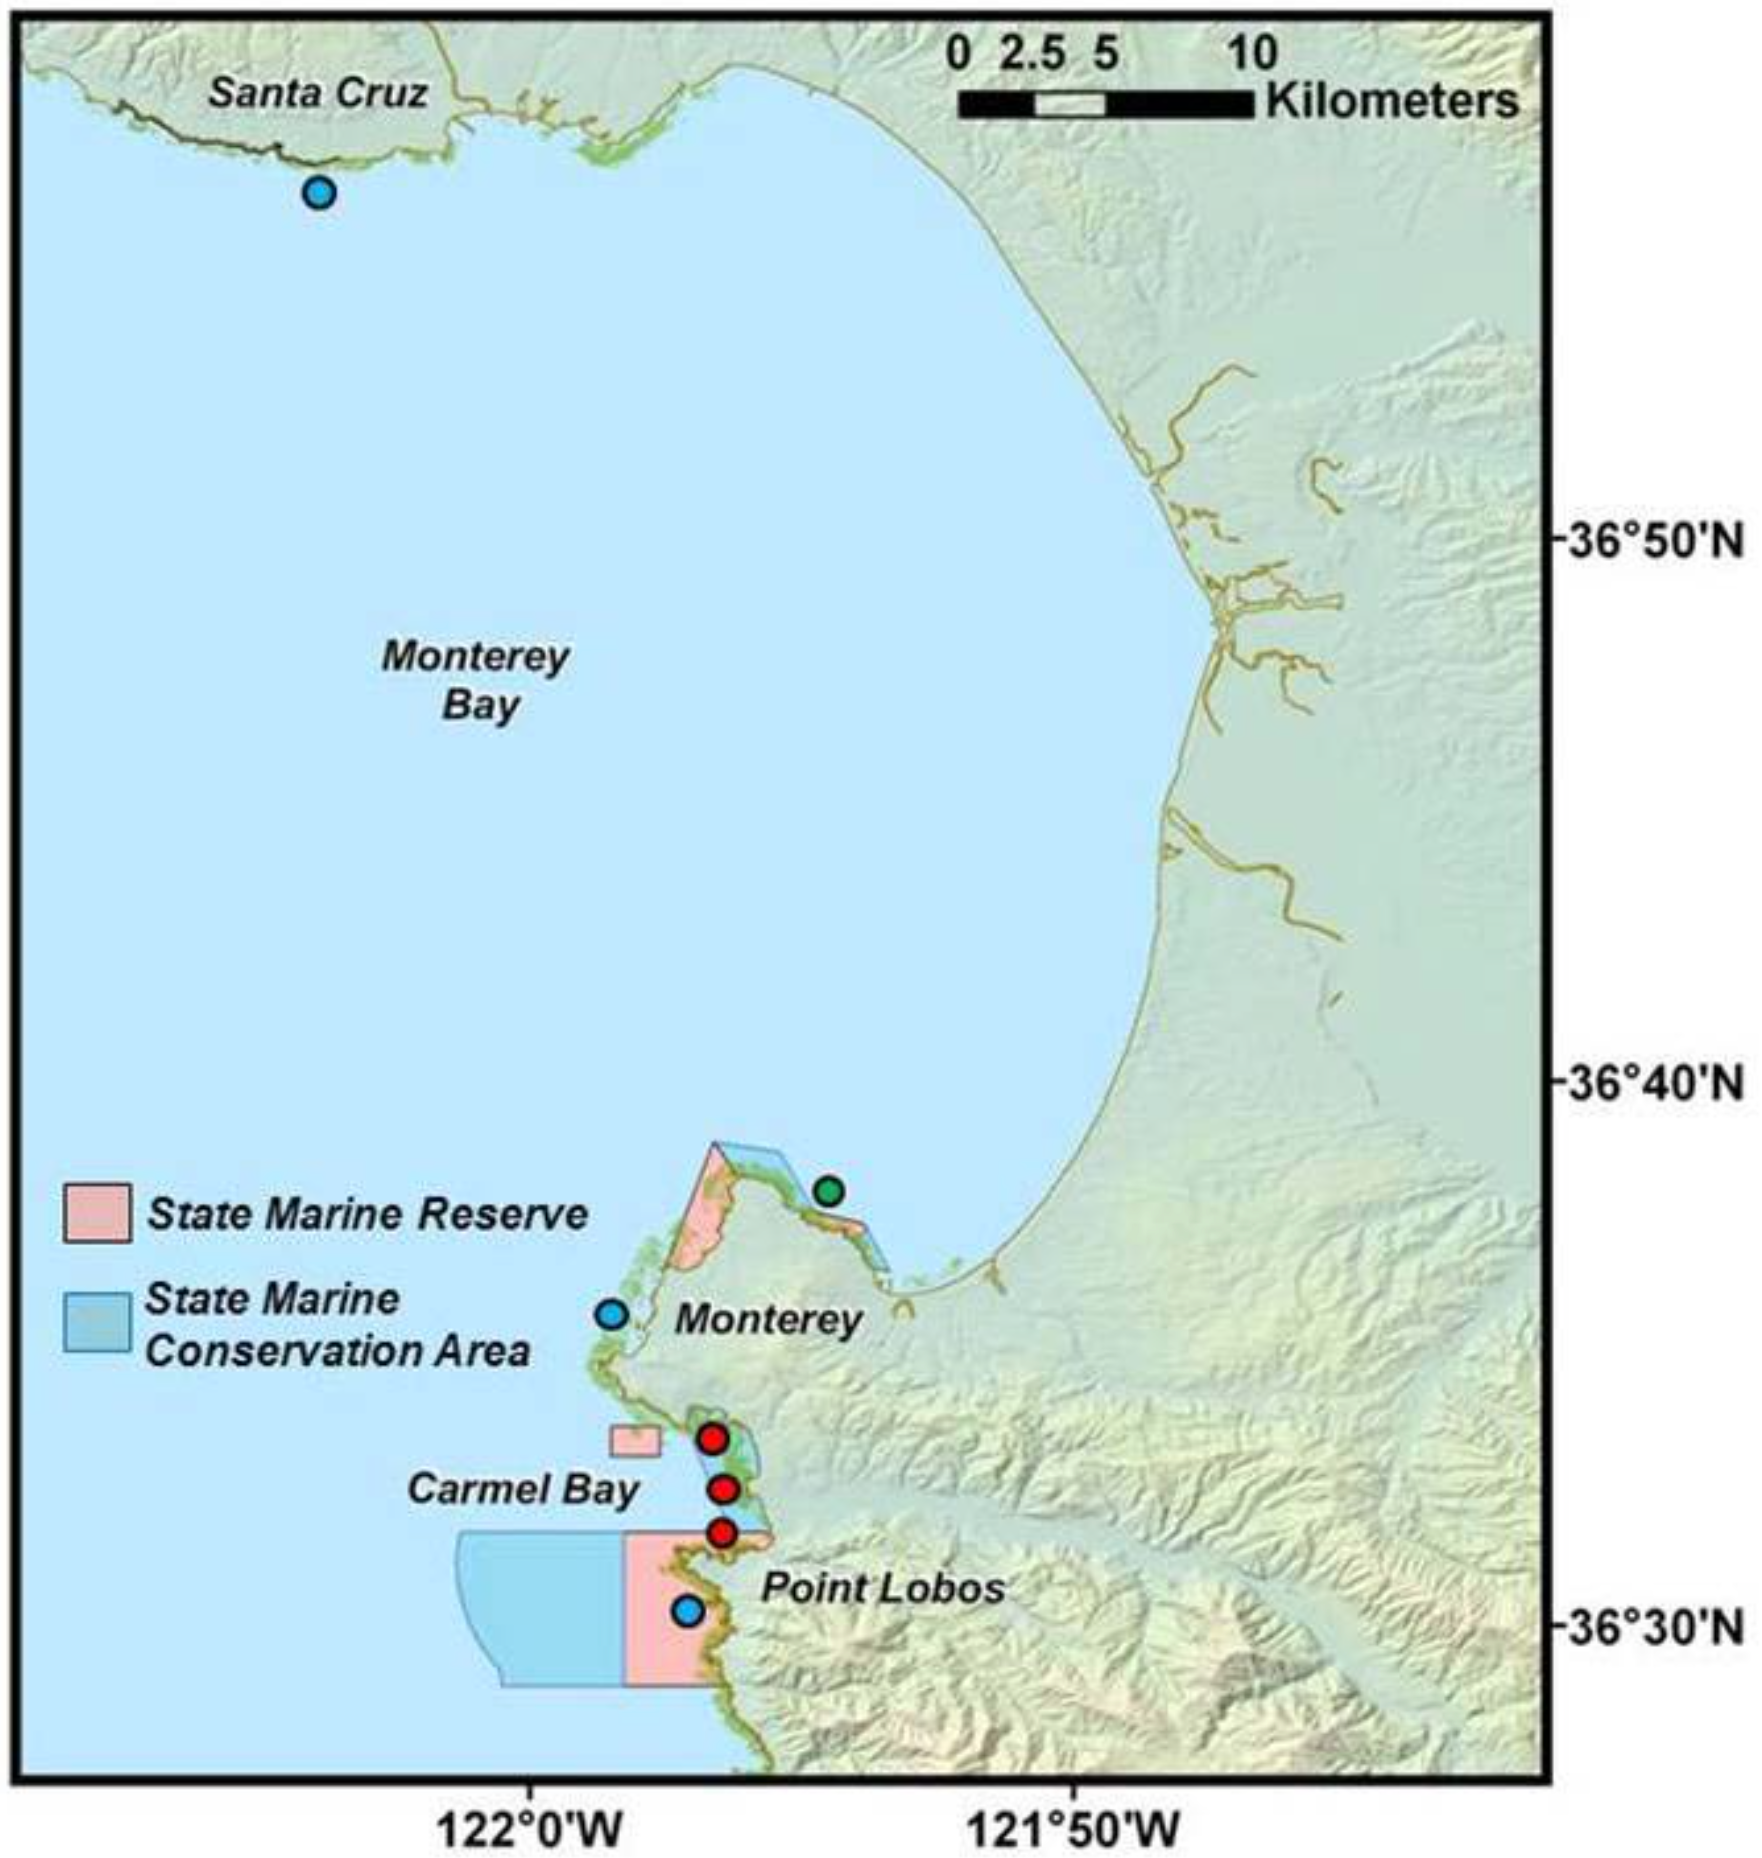
\includegraphics[width=.7\textwidth]{./figs/carmel_bay.png}\\
\end{center}
\end{frame}



\begin{frame}{SMURF traps}
\framesubtitle{Standard Monitoring Unit for the Recruitment of Reef Fishes}
\begin{center}
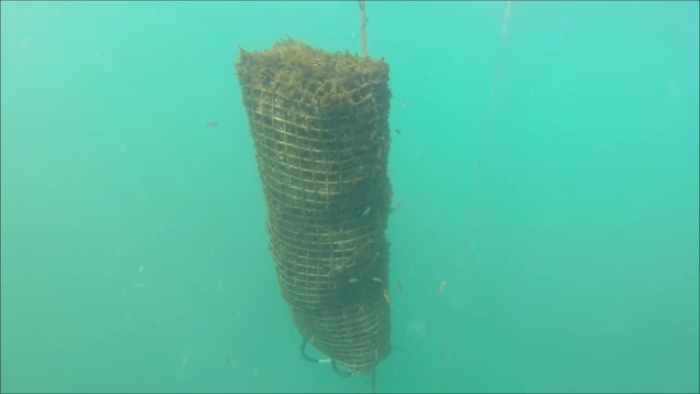
\includegraphics[width = 0.85\textwidth]{mhap_figs/smurf-solo.png}\\
{\tiny Carr-Raimondi lab photo}
\end{center}
\end{frame}



\begin{frame}{SMURF traps}
\framesubtitle{Standardized protocol for juvenile collection}
\begin{center}
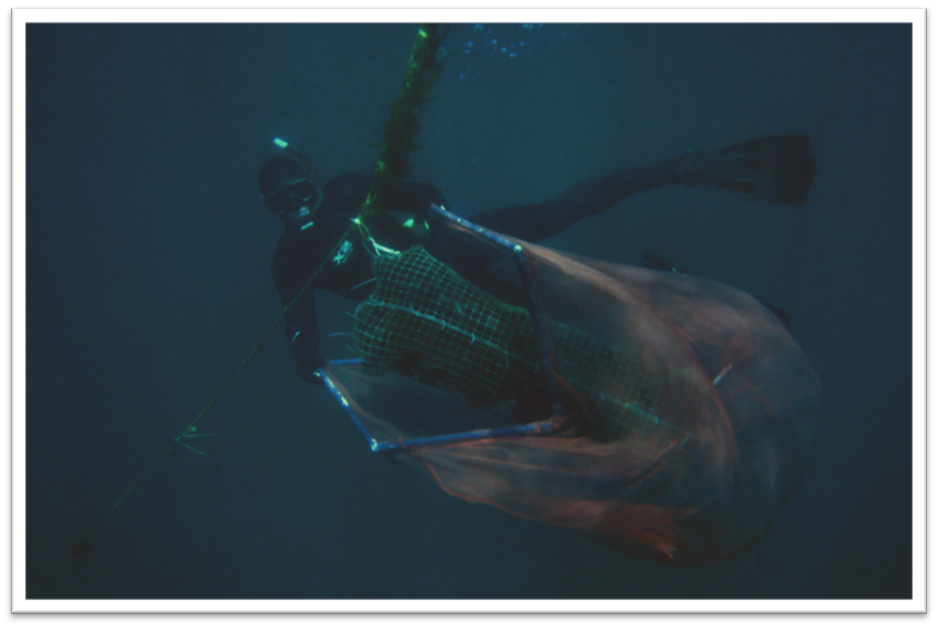
\includegraphics[width = 0.85\textwidth]{mhap_figs/smurf-binkie.png}\\
{\tiny Carr-Raimondi lab photo}
\end{center}
\end{frame}





\begin{frame}{Sampling of adult and juvenile rockfish}

\vspace*{-8ex}
Legions of undergraduates fishing and on SCUBA using biopsy-dart pole spears
\begin{center}
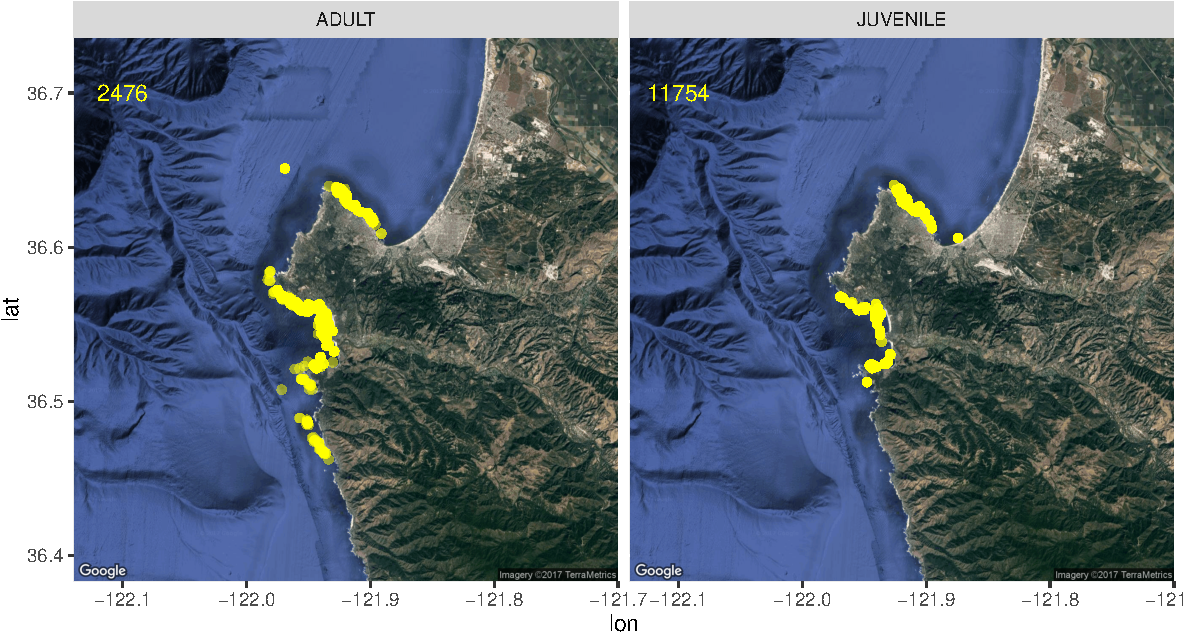
\includegraphics[width=\textwidth]{figs/sampling_map1-crop.pdf}
\end{center}

\mbox{}
\vspace*{-10ex}\mbox{}
Emily Saarman~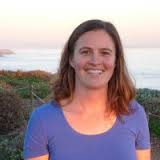
\includegraphics[height=.1\textheight]{figs/emily_saarman.jpg}
~~Dan Malone~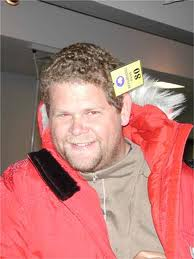
\includegraphics[height=.1\textheight]{figs/dan_malone.jpg}

\end{frame}





\begin{frame}{Genetic Sampling/Genotyping Goals}
\begin{itemize}
\item Across 3 to 4 years (and perhaps more if we can continue this) get non-lethal samples from $\approx$~5,000 adults and $\approx$~5,000 recruiting kelp rockfish. 
\item Accurately identify parent offspring pairs from amongst the 25 million possible pairs.
\item That is a lot of chances to make a mistake!  Why did we think we could do this?
\end{itemize}
\end{frame}






\begin{frame}{Digression: Why did we think we could do this?}
\framesubtitle{We had pioneered similar techniques for replacing Coded Wire Tags 
for the monitoring of hatchery salmon populations}
\begin{center}
\mbox{}
\hfill
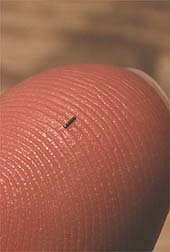
\includegraphics[height=.33\textwidth]{./figs/finger.jpg}
\hfill
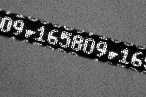
\includegraphics[height=.2\textwidth]{./figs/cwt.png}
\hfill
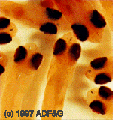
\includegraphics[height=.25\textwidth]{./figs/pink.png}
\hfill
\mbox{}
\end{center}
Our lab routinely genotypes tens of thousands of fish each year.
\end{frame}



\begin{frame}{Originally-proposed approach}
\framesubtitle{Large-scale parentage inference with microfluidic SNP assays}
\begin{center}
\mbox{}\hspace*{-.10\textwidth}
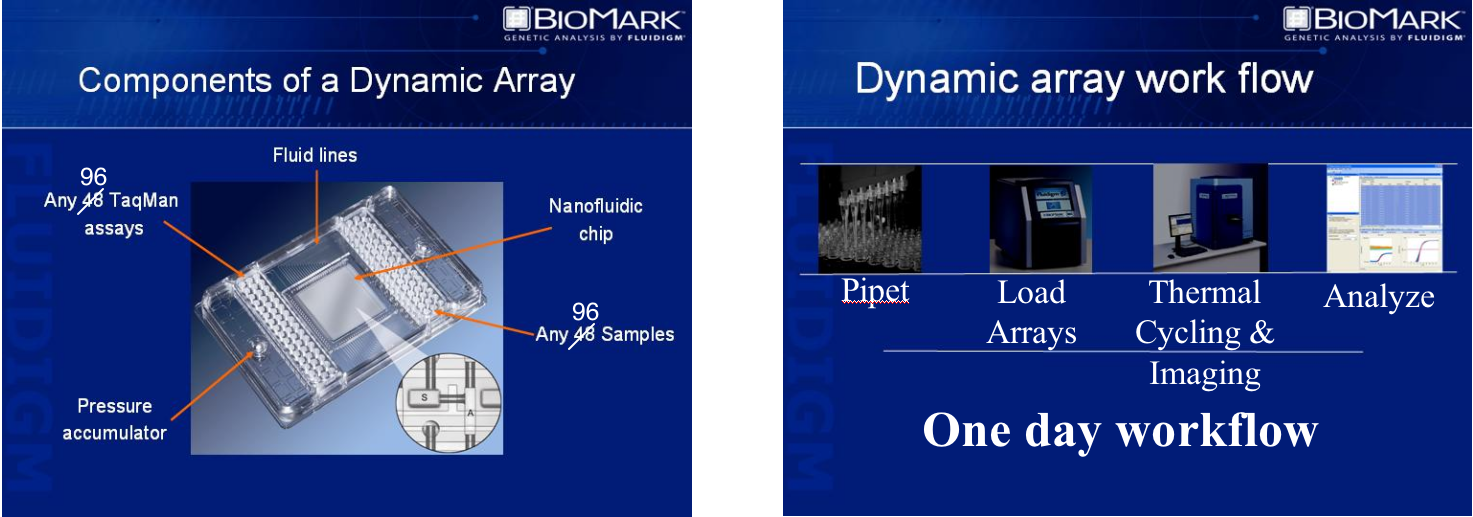
\includegraphics[width=1.16\textwidth]{figs/fluidigm.png}\\
With 96.96 Arrays and only one controller and thermal cycler, \\
can genotype almost 300 fish per day w/96 SNPs.

Cost: $<$\$10/fish 
\end{center}
\end{frame}








\begin{frame}{Microfluidic chips, a known quantity}
\begin{center}
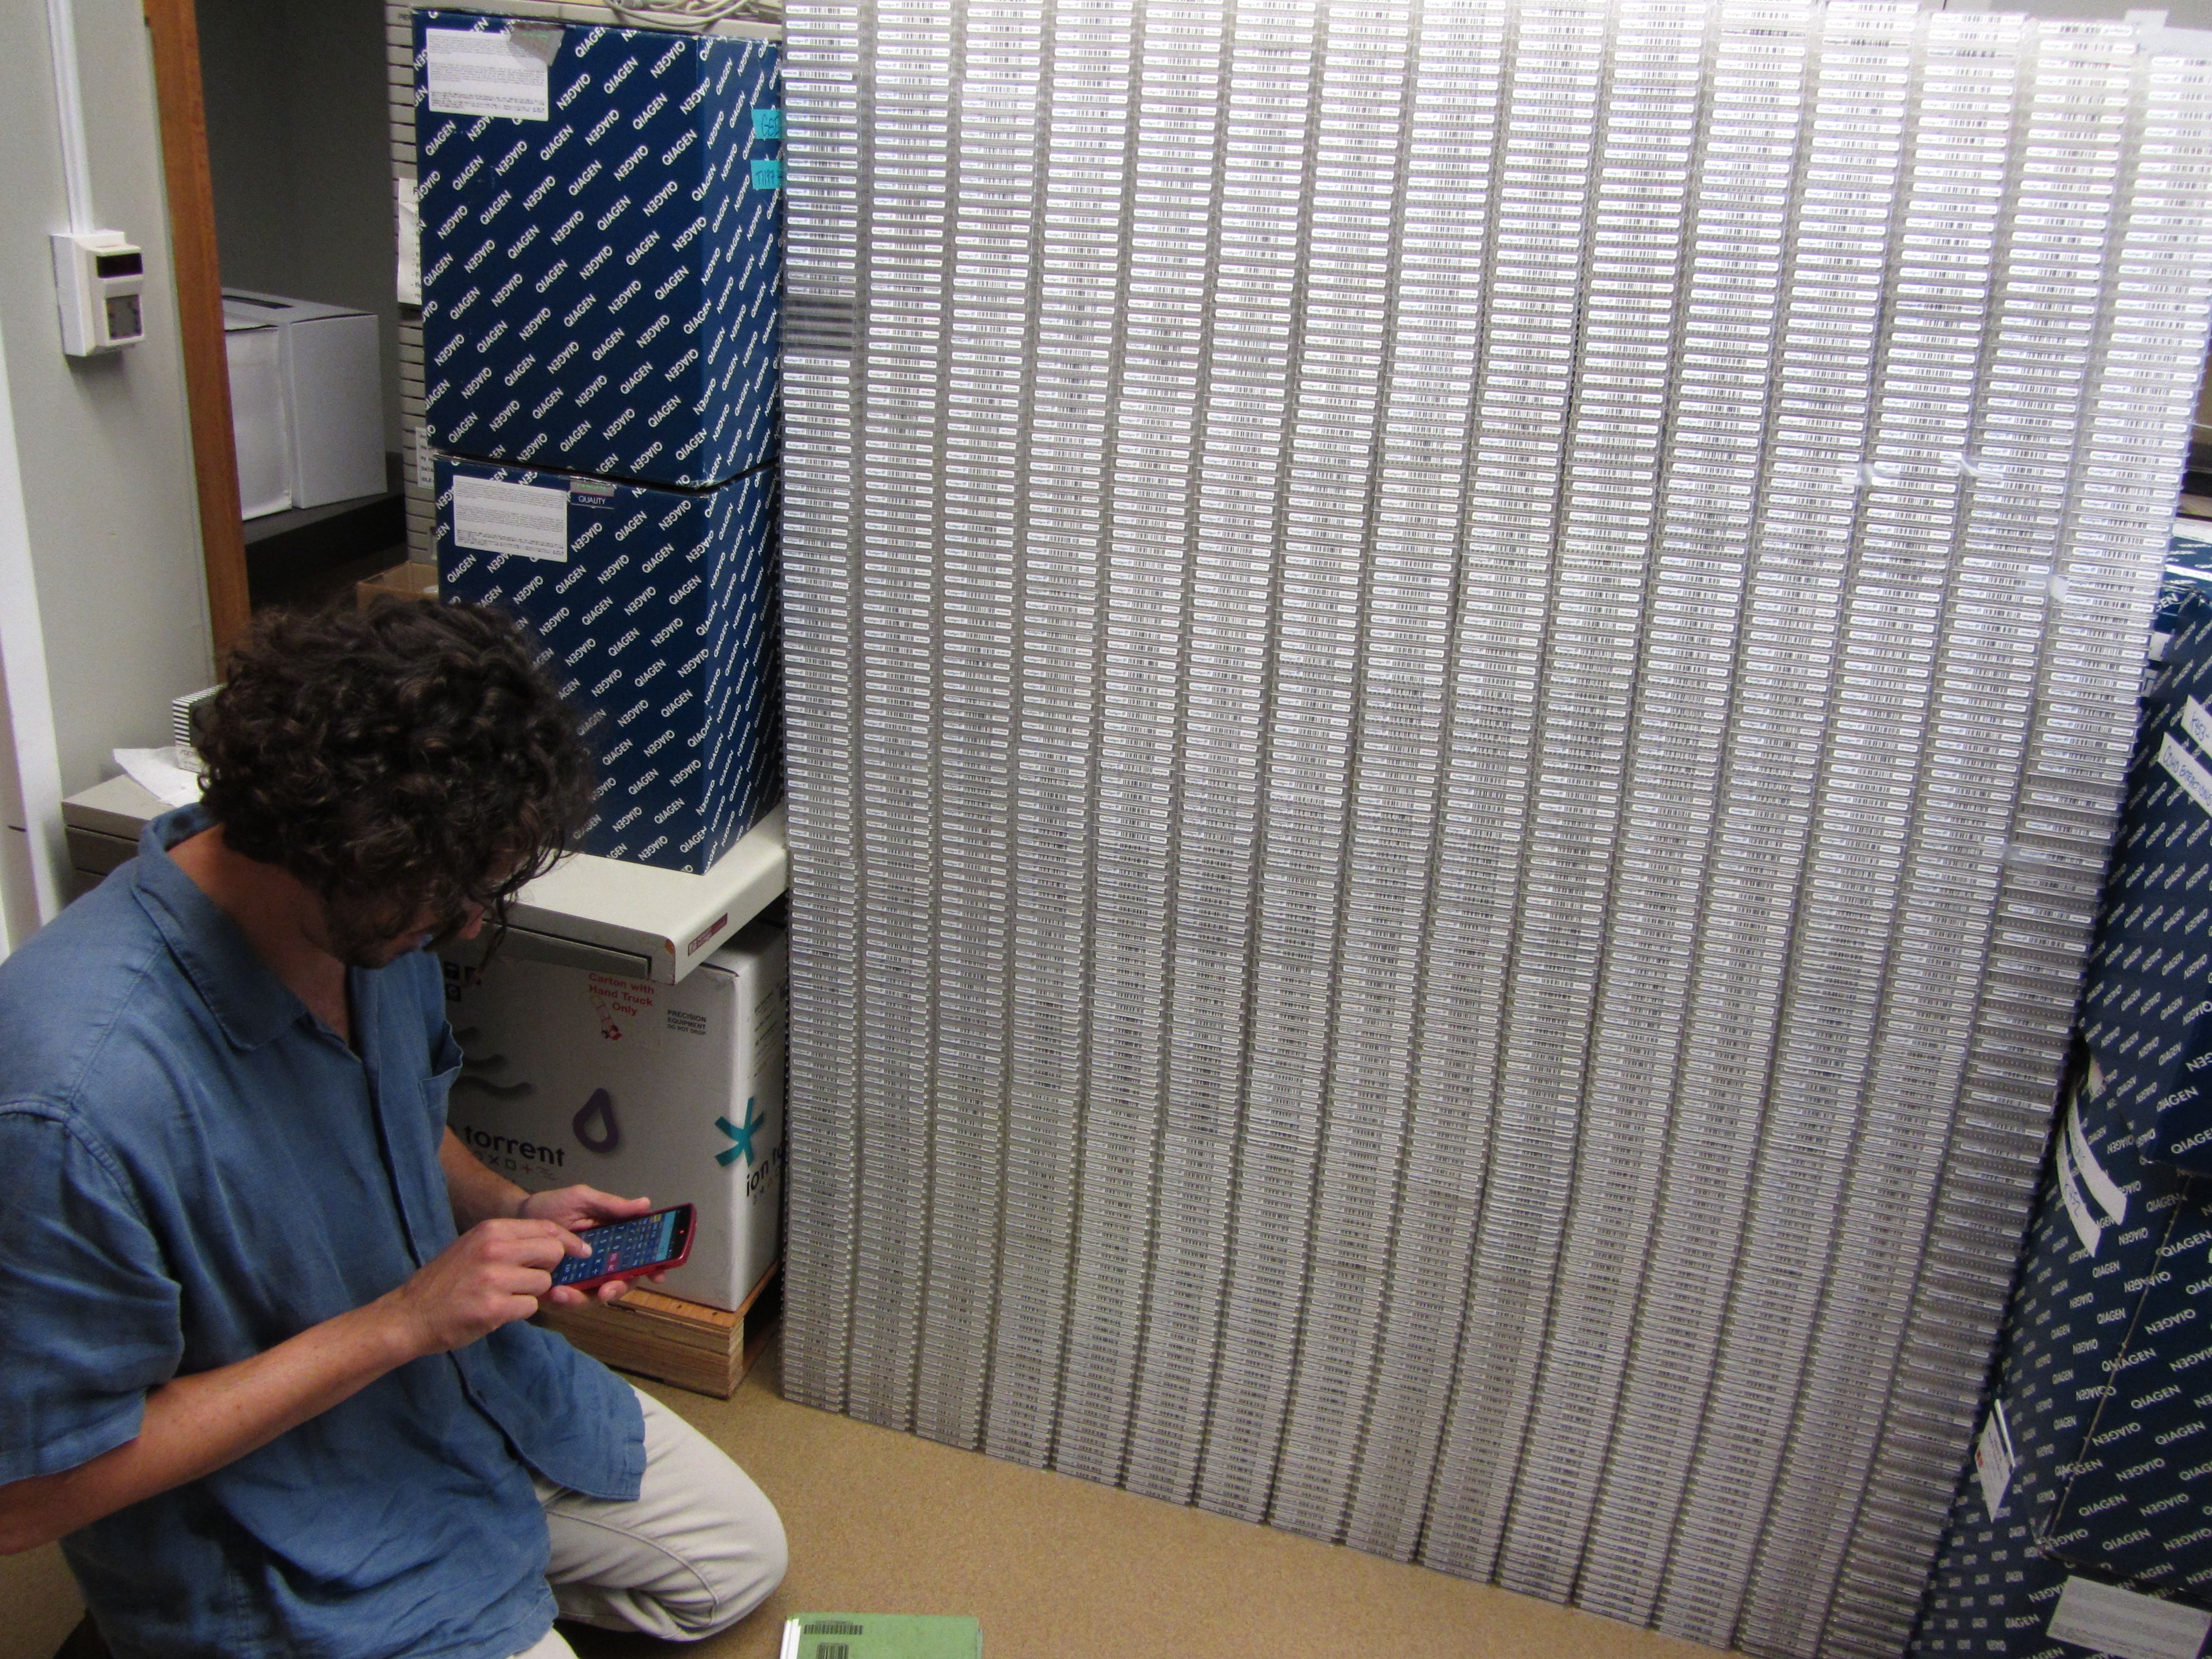
\includegraphics[width=0.75\textwidth]{figs/AC_calculating_chipwall.jpg}
\end{center}
$\bullet$ However, 96 SNPs are not enough for single parent assignments,\\
$\bullet$ and species ID in juveniles is unreliable
\end{frame}





\begin{frame}{The juvenile ID bombshell}
\begin{columns}
\begin{column}{.38\textwidth}
\includegraphics[width=\textwidth]{./figs/juvie_rockfish.png}
\end{column}
\begin{column}{.55\textwidth}
\begin{itemize}
\item Below a certain size, kelp, gopher, and black-and-yellow rockfish are not visually dinstinguishable.
\item Upwards of 50\% of juveniles could be non-kelp!
\item Non-kelp rockfish could be identified with our SNP assay
\item But, the SNP data on those other species would be essentially worthless
\item Solution: hijack NGS tech to create markers useful for all three species
\end{itemize}


\end{column}

\end{columns}

\end{frame}






\begin{frame}{Next Generation Sequencing -- I}
\framesubtitle{Illumina Sequencing By Synthesis}
{\centering
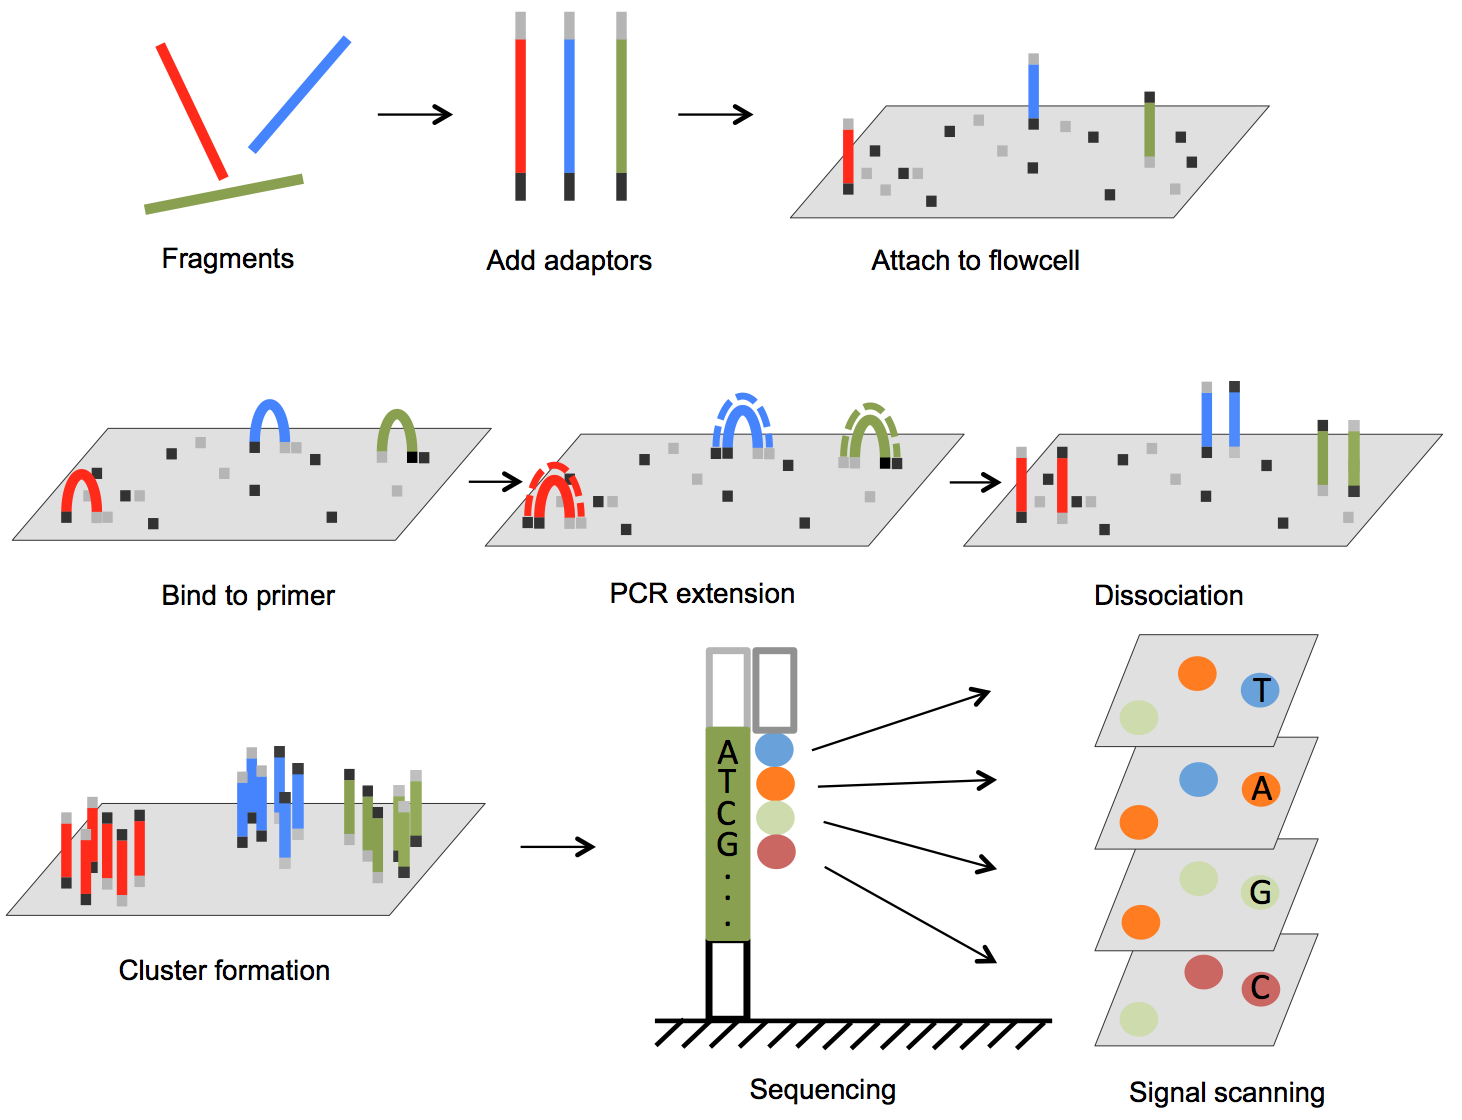
\includegraphics[height=0.80\textheight]{mhap_figs/illumina_fig.png}
}\\
{\tiny http://www.intechopen.com}
\end{frame}







\begin{frame}{Next Generation Sequencing -- II}
\framesubtitle{{\em de novo} ``genome'' assembly}
{\centering
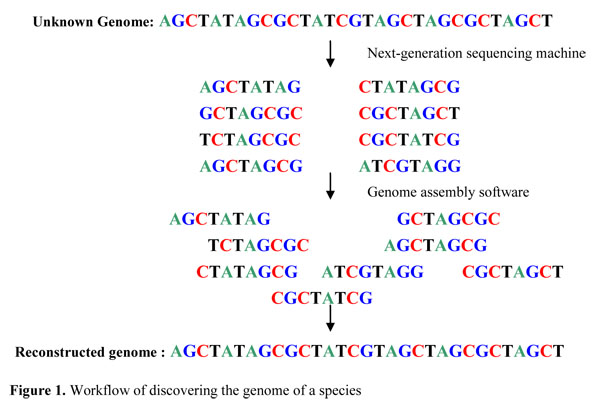
\includegraphics[height=0.75\textheight]{mhap_figs/assembly.png}
}\\
{\tiny http://www.cs.hku.hk}
\end{frame}






\begin{frame}{Next Generation Sequencing -- III}
\framesubtitle{Alignment of sequencing reads to ``genome'' allows \\
identification of polymorphisms and genotyping}
{\centering
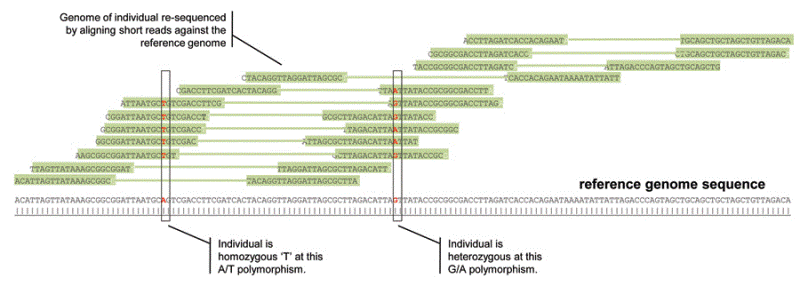
\includegraphics[width=0.95\textwidth]{mhap_figs/alignment.png}
}\\
{\tiny http://www.historyofnimr.org.uk}
\end{frame}






\begin{frame}{GTseq amplicon sequencing}
\begin{center}
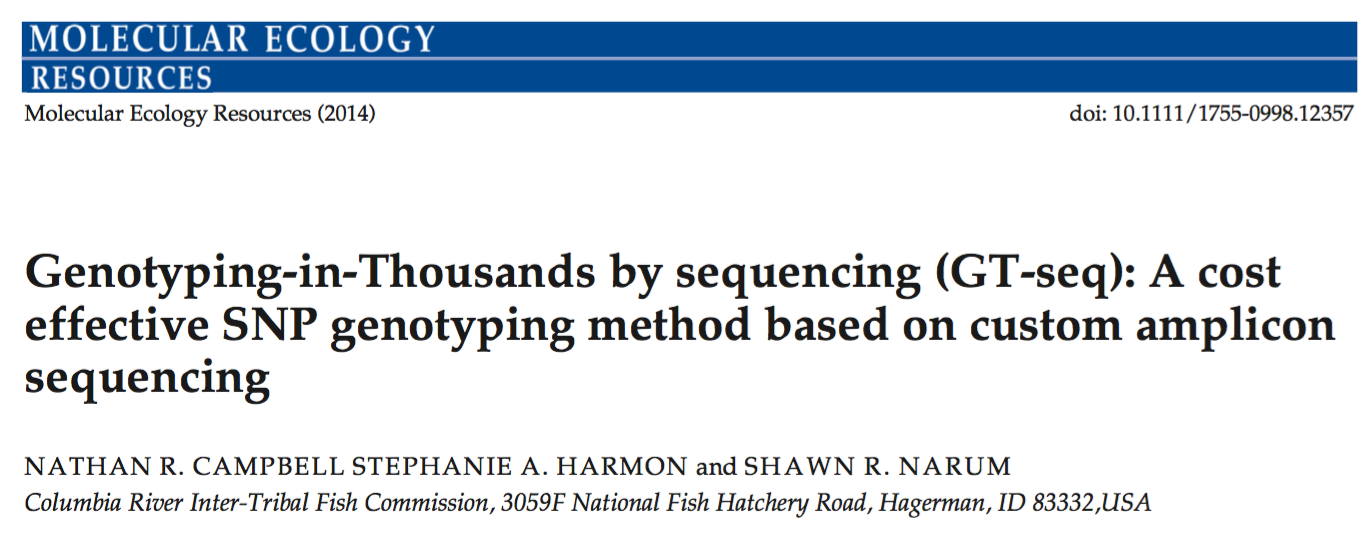
\includegraphics[width=0.95\textwidth]{figs/gtseq-header.png}
\end{center}
\begin{itemize}
\item Multiplexed PCR primers amplify regions of interest.
\item Amplicon sequencing of 100--500 regions in 300--2,000 individuals
\item $\approx \$7$/individual
\item Converted Fluidigm SNP assays.  Tens of 1,000s of salmon each year.
\end{itemize}
\end{frame}








\begin{frame}{GTseq -- I {\small (coming off the sequencer\ldots)}}
\framesubtitle{2 Amplicons; 3 individuals on each of 3 plates (9 individuals total)}
\begin{center}
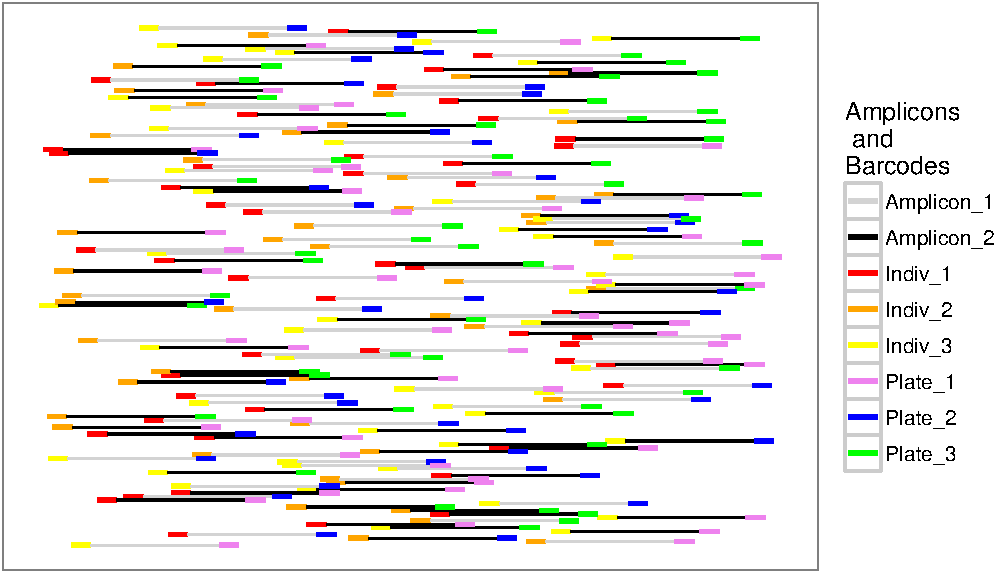
\includegraphics[width=0.95\textwidth]{figs/gtseq-soup-crop.pdf}
\end{center}
\end{frame}





\begin{frame}{GTseq -- II (aligned amplicons)}
\framesubtitle{Amplicon sequences are known. Alignment {\em in silico} is straightforward.}
\begin{center}
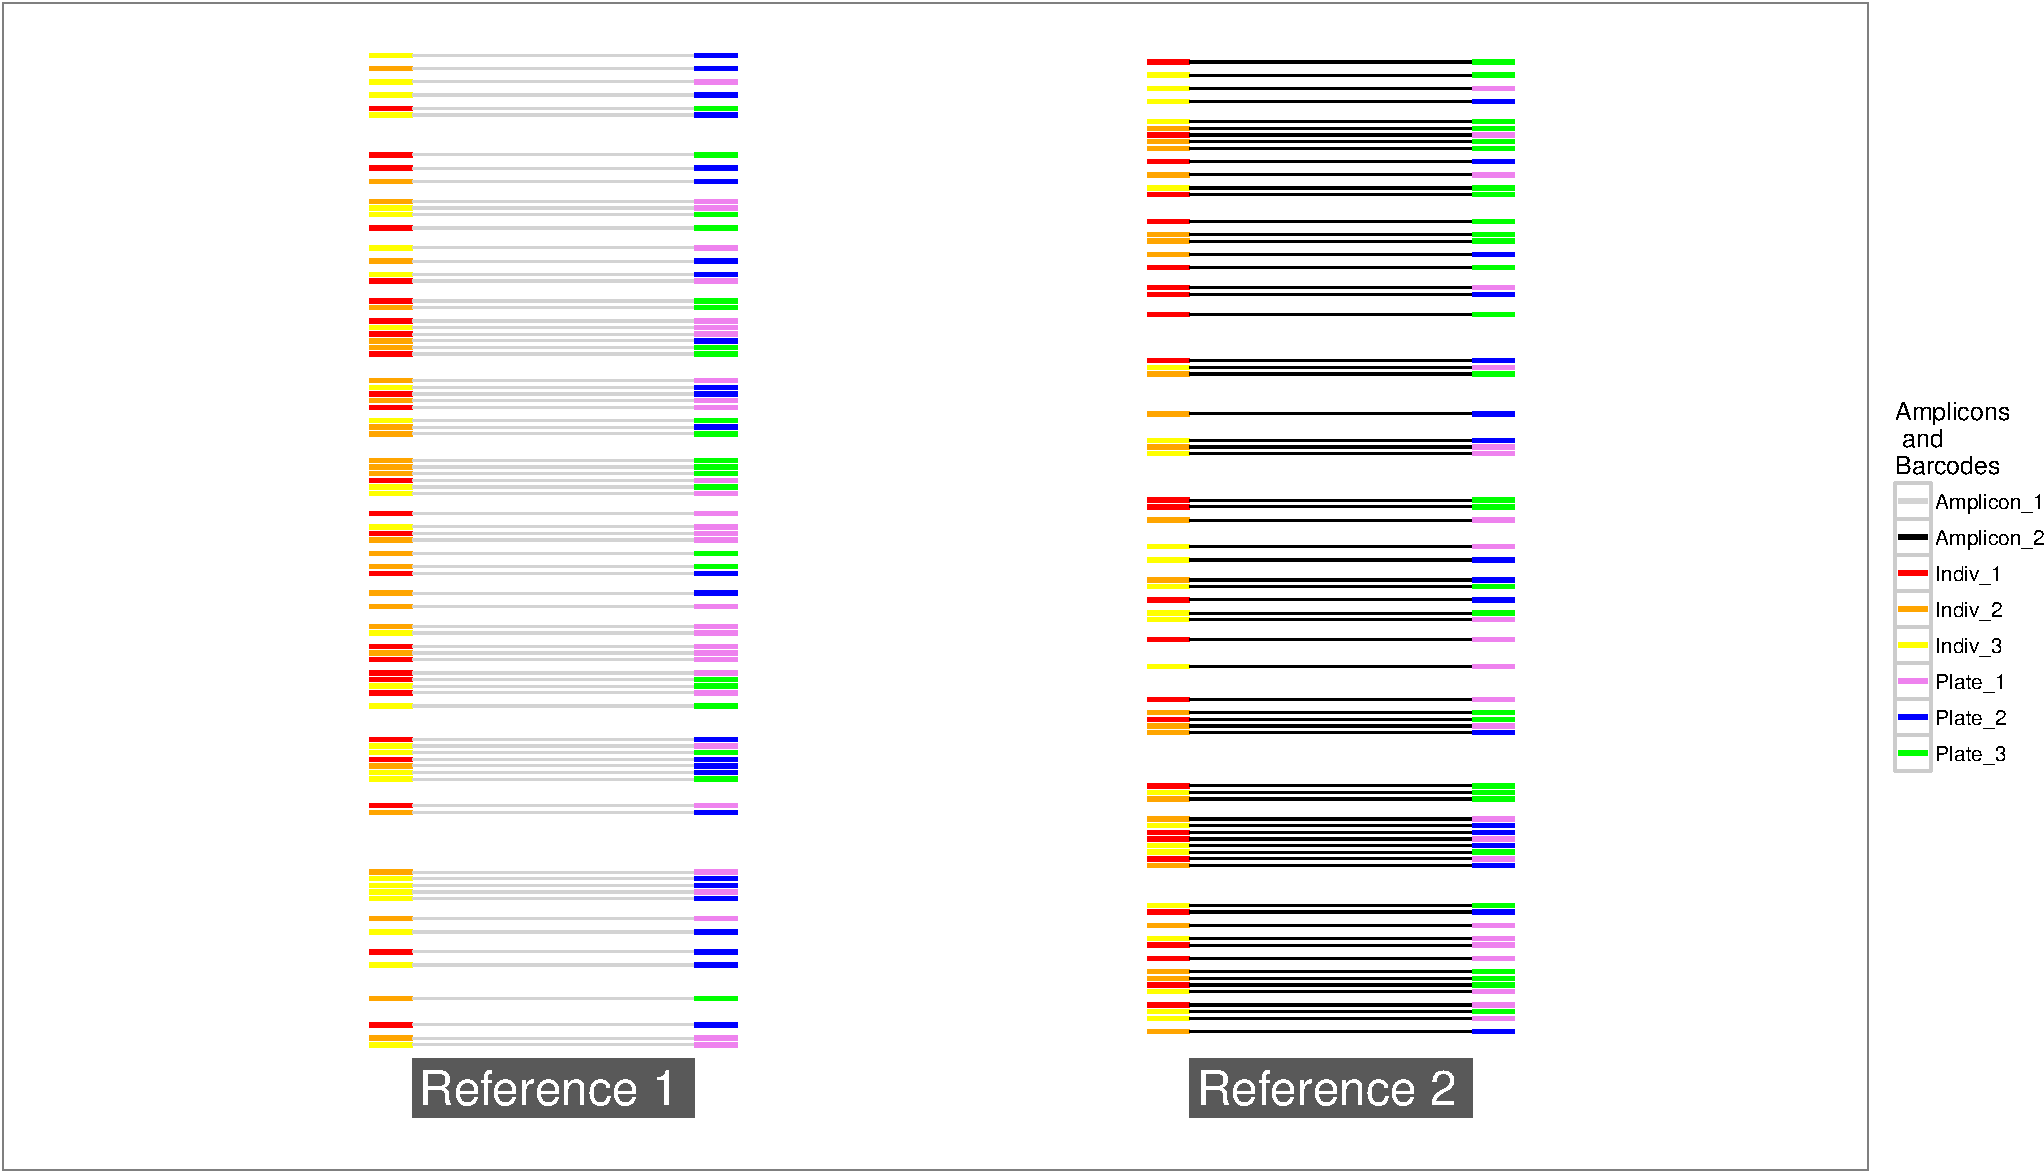
\includegraphics[width=0.95\textwidth]{figs/gtseq-amps-crop.pdf}
\end{center}
\end{frame}



\begin{frame}{GTseq -- III (``demultiplexing'')}
\framesubtitle{Identify individual origin of reads via combinatorial barcodes}
\begin{center}
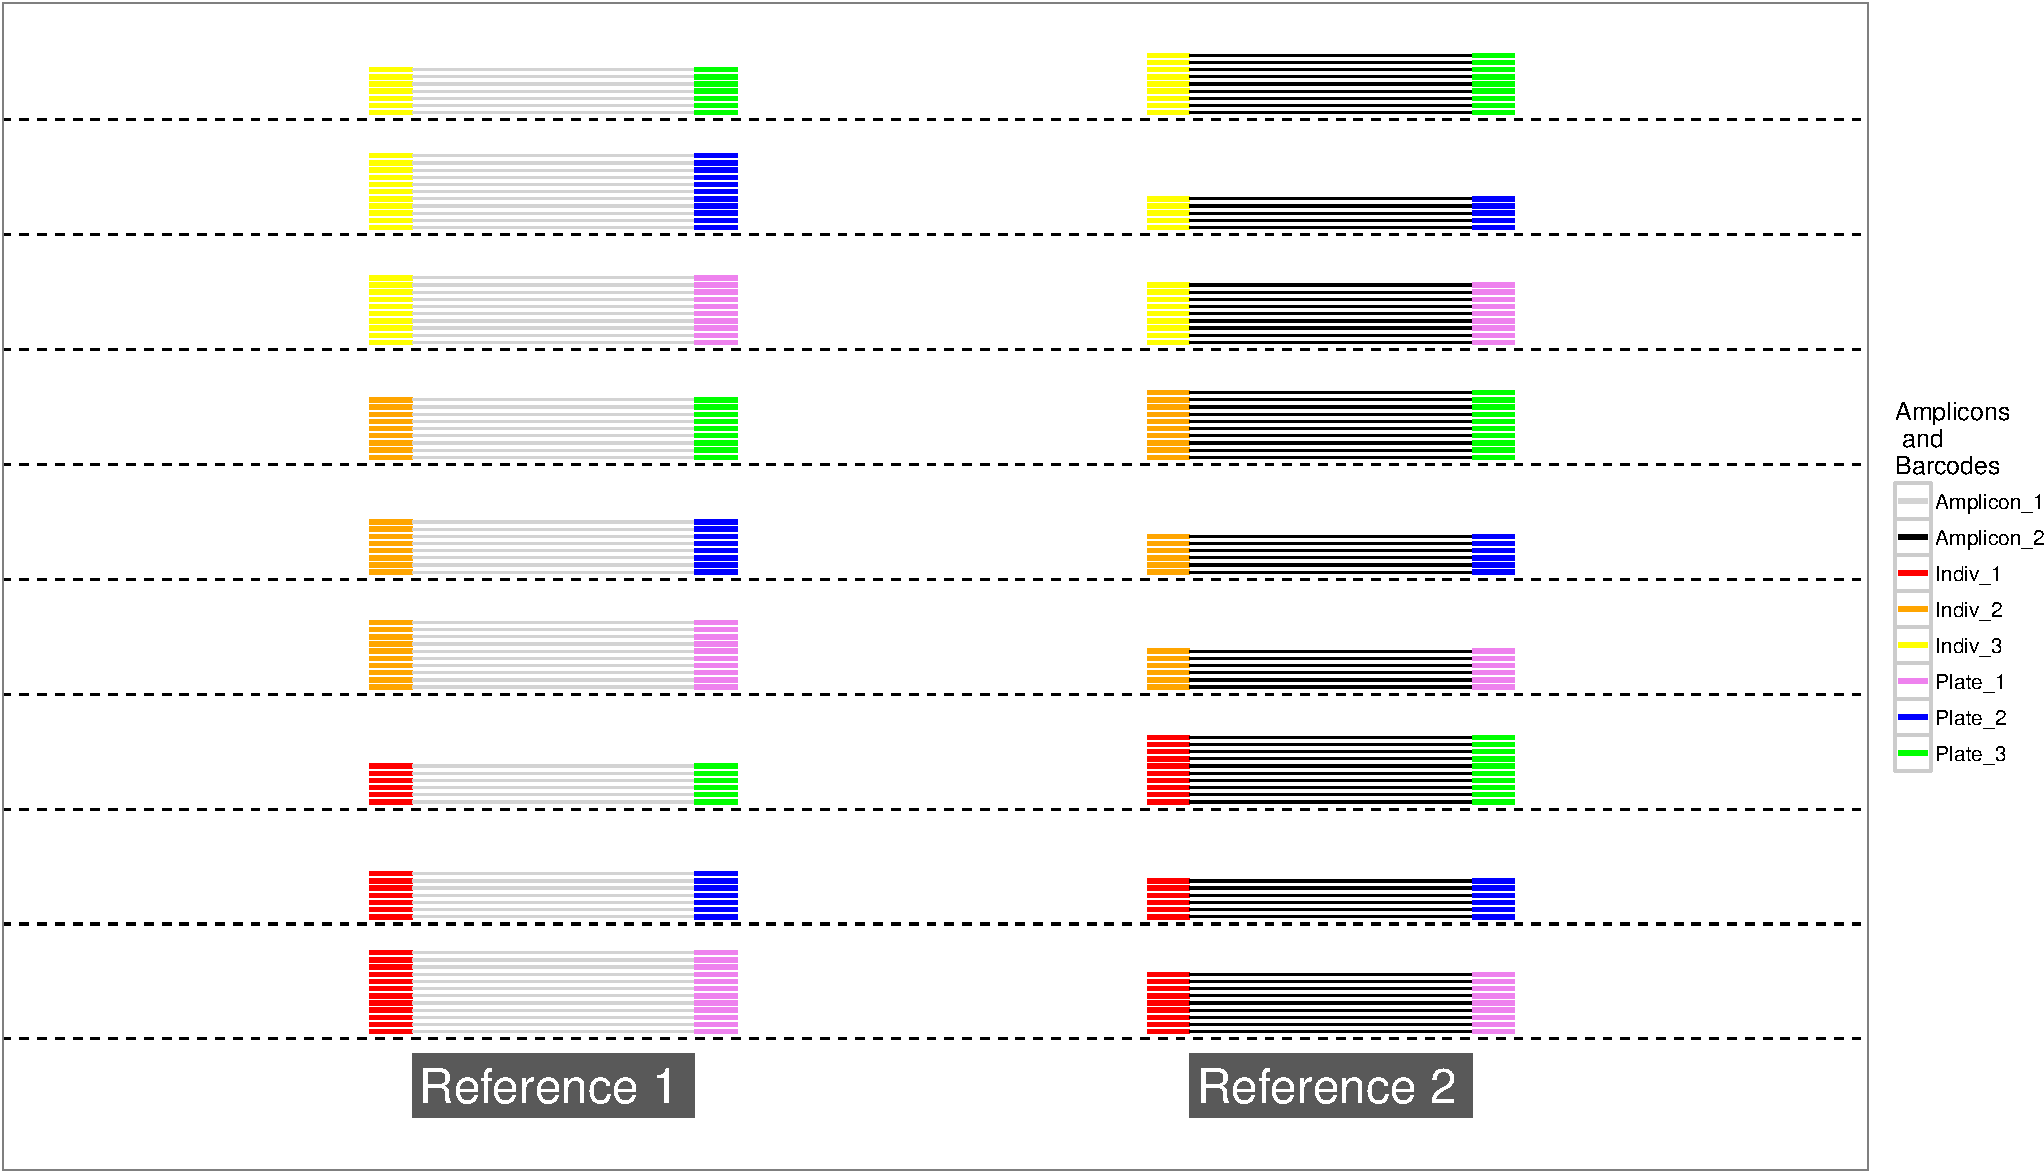
\includegraphics[width=0.95\textwidth]{figs/gtseq-demultiplexed-crop.pdf}
\end{center}
\end{frame}





\begin{frame}{GTseq -- IV (identify SNPs in sequence)}
\framesubtitle{Variants are easy to identify}
\begin{center}
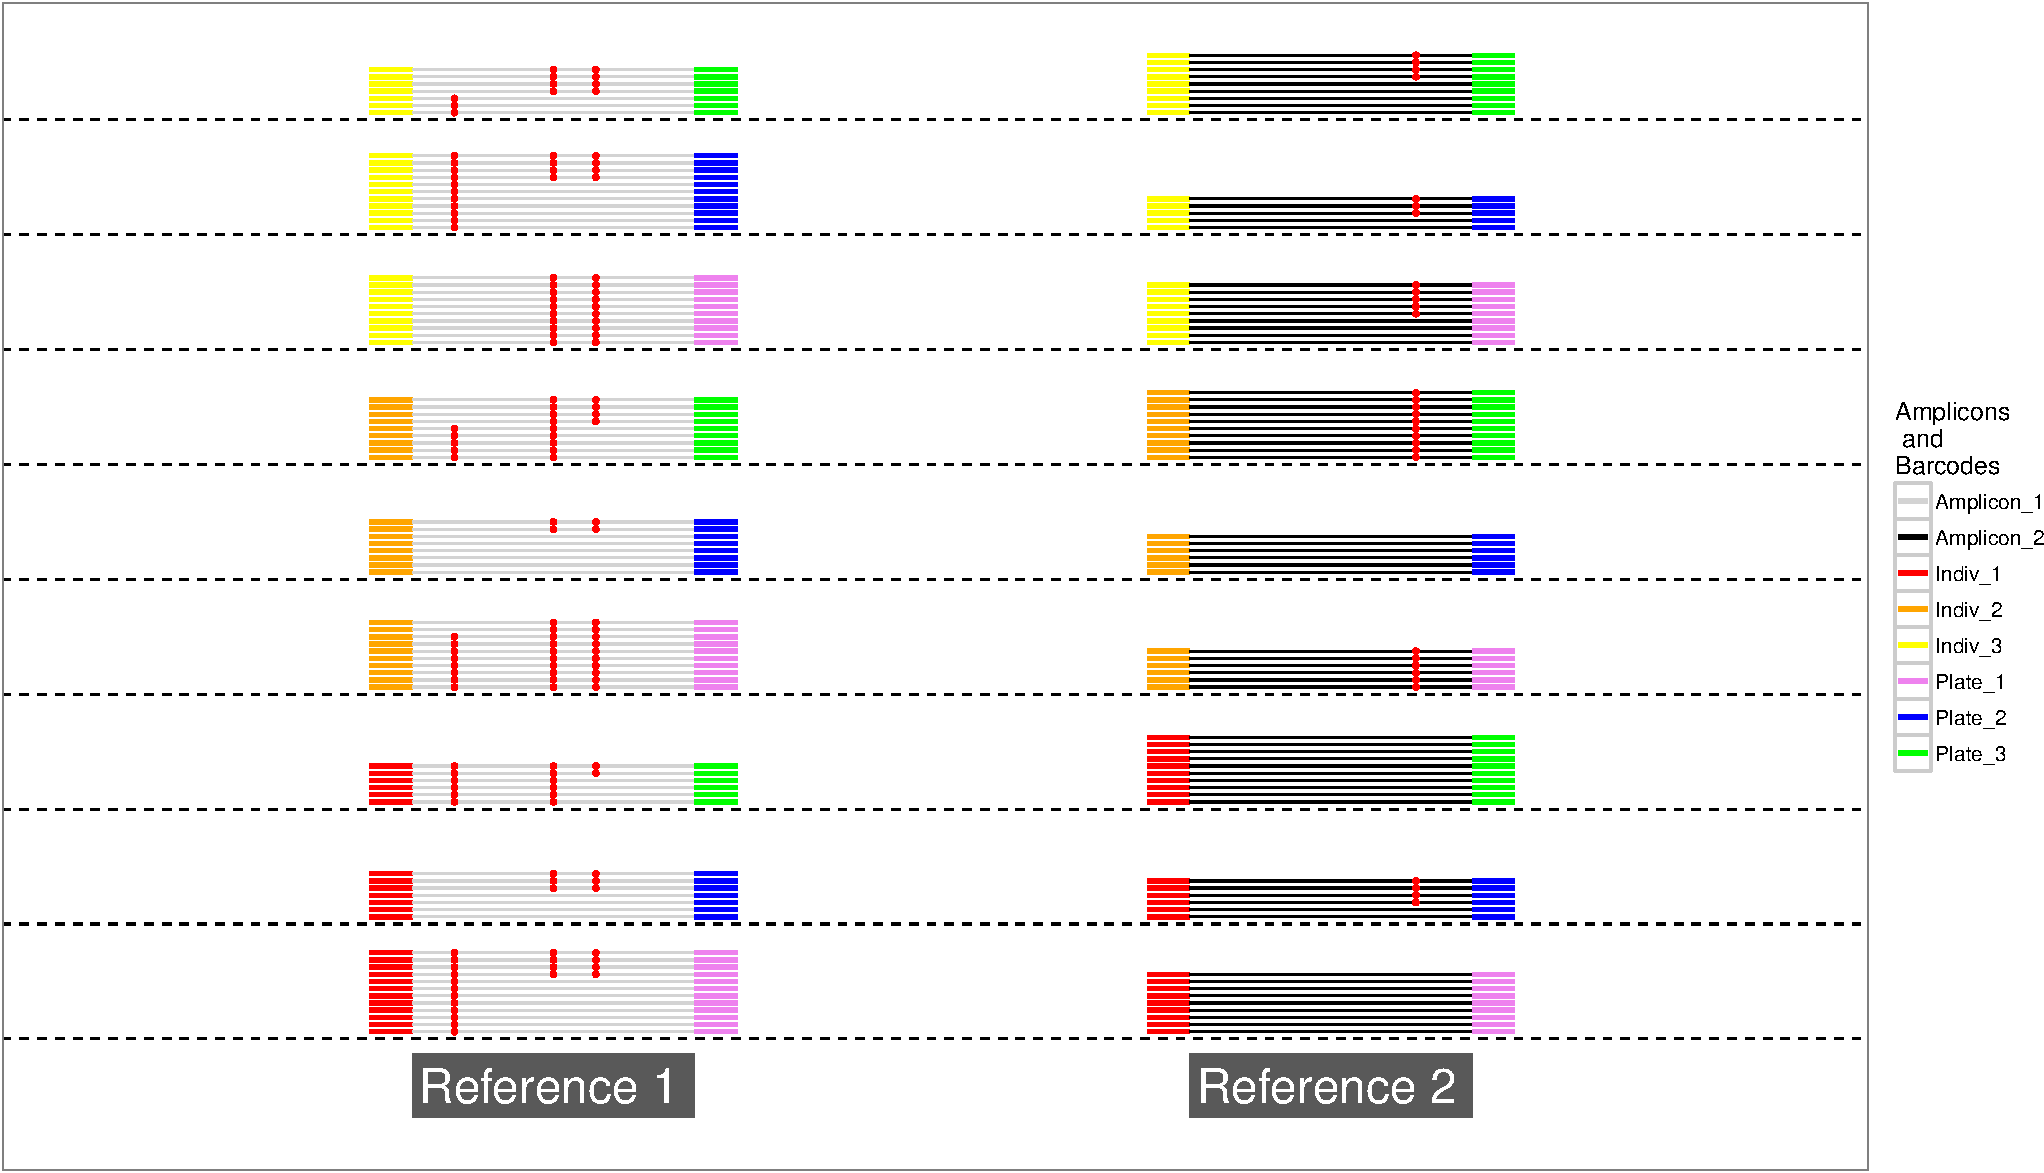
\includegraphics[width=0.95\textwidth]{figs/gtseq-snps-crop.pdf}
\end{center}
\end{frame}




\begin{frame}{Multiple SNPs in amplicons/sequences\ldots}
\framesubtitle{\ldots are almost universally ignored }
\begin{itemize}
\item Multiple SNPs in each amplicon/RAD-locus are typically scored
\item But then either:
\begin{enumerate}
\item Only a single SNP from each amplicon/locus is used
\item OR, all SNPs are treated as unlinked
\end{enumerate}
Depending on the analyses, the result is either a lack of power or (potentially) incorrect inference.
\end{itemize}
\end{frame}






\begin{frame}{Phase of SNPs on reads is almost universally ignored}
\begin{center}
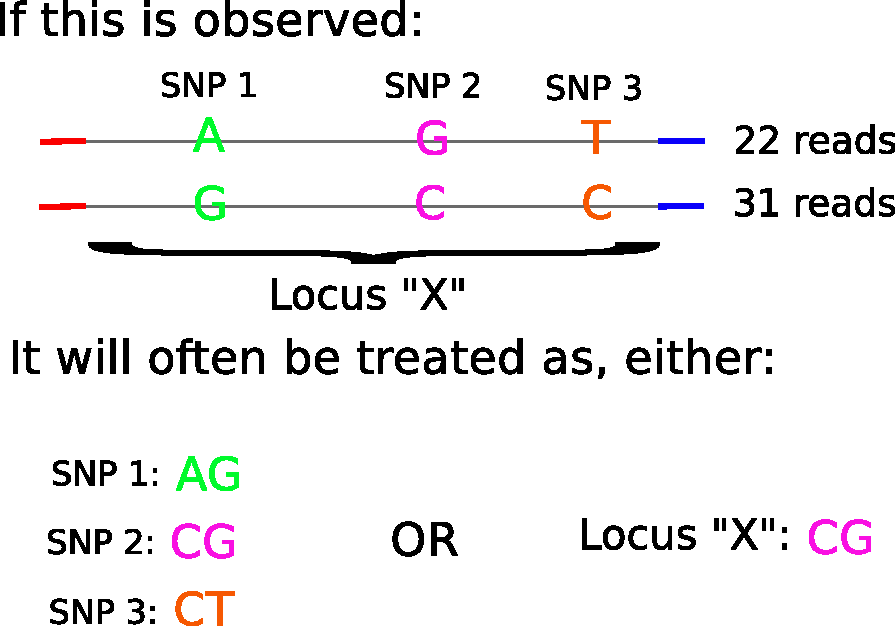
\includegraphics[width=0.94\textwidth]{figs/three-snp-reads.pdf}
\end{center}
\end{frame}













\begin{frame}{Microhaplotypes}
\framesubtitle{A simple idea / plea, that\ldots}
\begin{center}
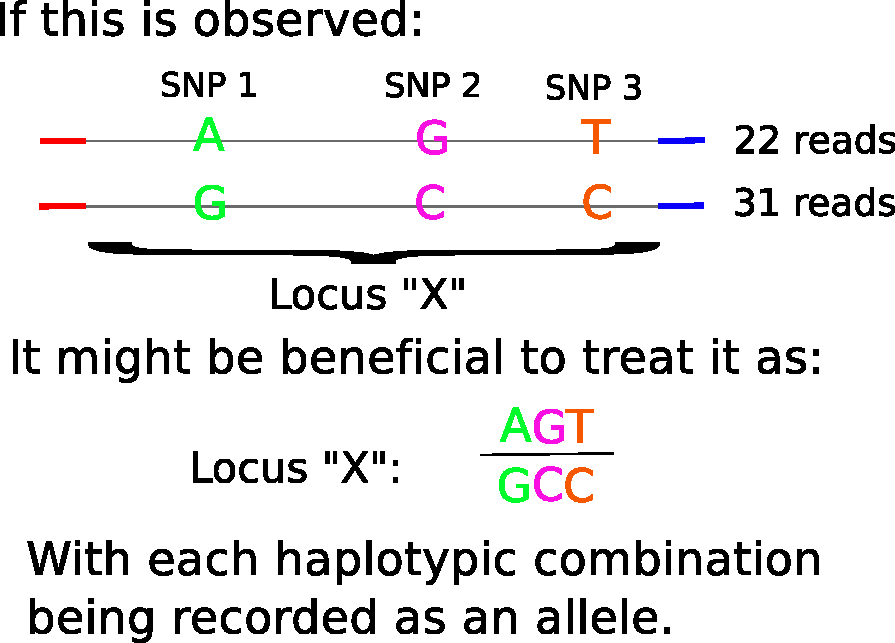
\includegraphics[width=0.94\textwidth]{figs/three-snp-reads-mhap.pdf}
\end{center}
\end{frame}






\begin{frame}{Microhaplotypes}
\framesubtitle{Potential advantages}
\begin{itemize}
\item Multiallelic loci
\begin{itemize}
\item More power for relationship inference / pedigree reconstruction
\end{itemize}
\item Need not discard SNPs from certain loci
\begin{itemize}
\item Retain low-frequency variants.  Useful for population structure in recently diverged populations.
\end{itemize}
\item Amplicons typically cross-amplify between closely-related species
\begin{itemize}
\item Unlike single SNP assays, the microhaplotype data collection method, unmodified,
can yield useful data for non-target species.
\item So, we opened up sampling to more species
\end{itemize}
\item We designed 96 microhaplotype amplicons for genotyping on an Illumina Mi-Seq in batches of 384 individuals.
\end{itemize}
\end{frame}










\begin{frame}{Microhaplotype Genotyping}
\framesubtitle{Whoa!  15,000 fish genotyped in $<$4 months. Total materials cost $\approx$\$6/fish}
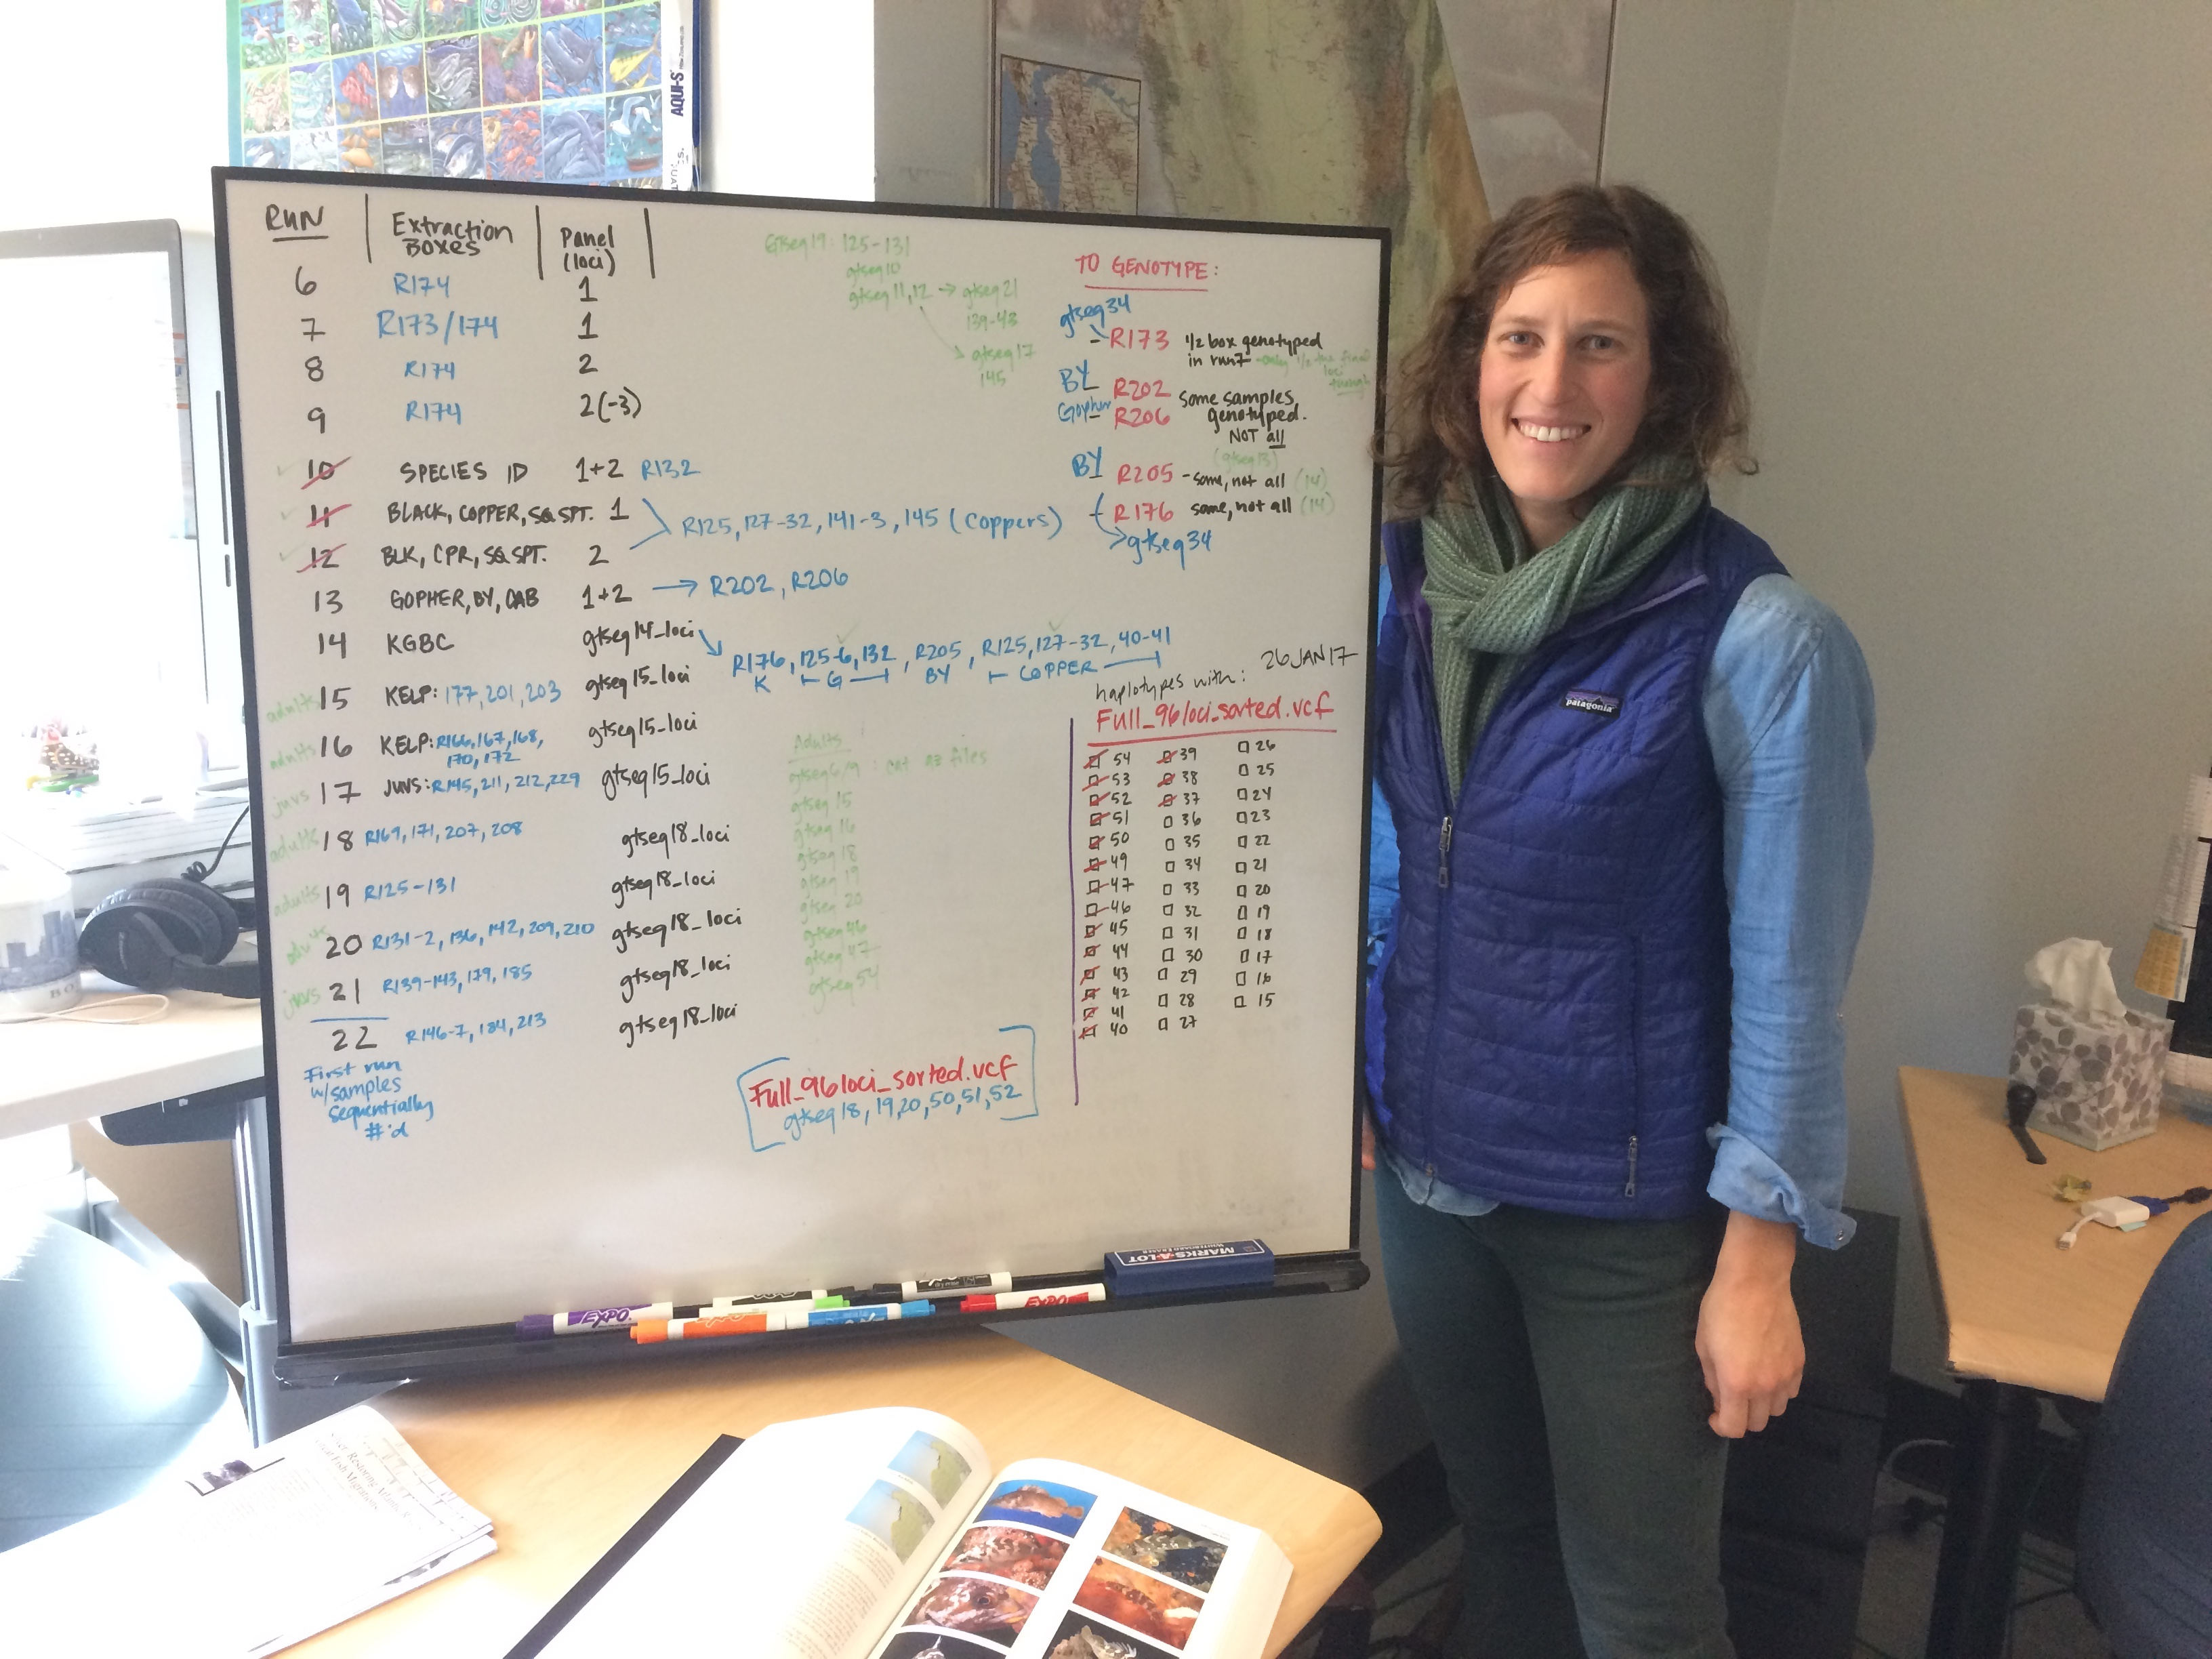
\includegraphics[width = 0.8\textwidth]{figs/diana.jpg}\\
{\footnotesize Diana Baetscher (UCSC Grad Student) }
\end{frame}




\begin{frame}{Extracting microhaplotypes from alignments}
\framesubtitle{Bioinformatics software from our lab --- {\sc microhaplot}}

\begin{columns}
\begin{column}{0.5\textwidth}
\begin{itemize}
{\small
\item R package by Thomas Ng (UCSC grad student)
\item Appoint SNPs in haplotypes with a VCF file
\item Extract haplotypes from SAM files
\item Filter on Read Depth / Allelic Balance ratio
\item Partially completed Bayesian inference of haplotypes
\item Full Shiny App for Visualization.
}
{\tiny https://github.com/ngthomas/microhaplot}
\end{itemize}
\end{column}
\begin{column}{0.5\textwidth}
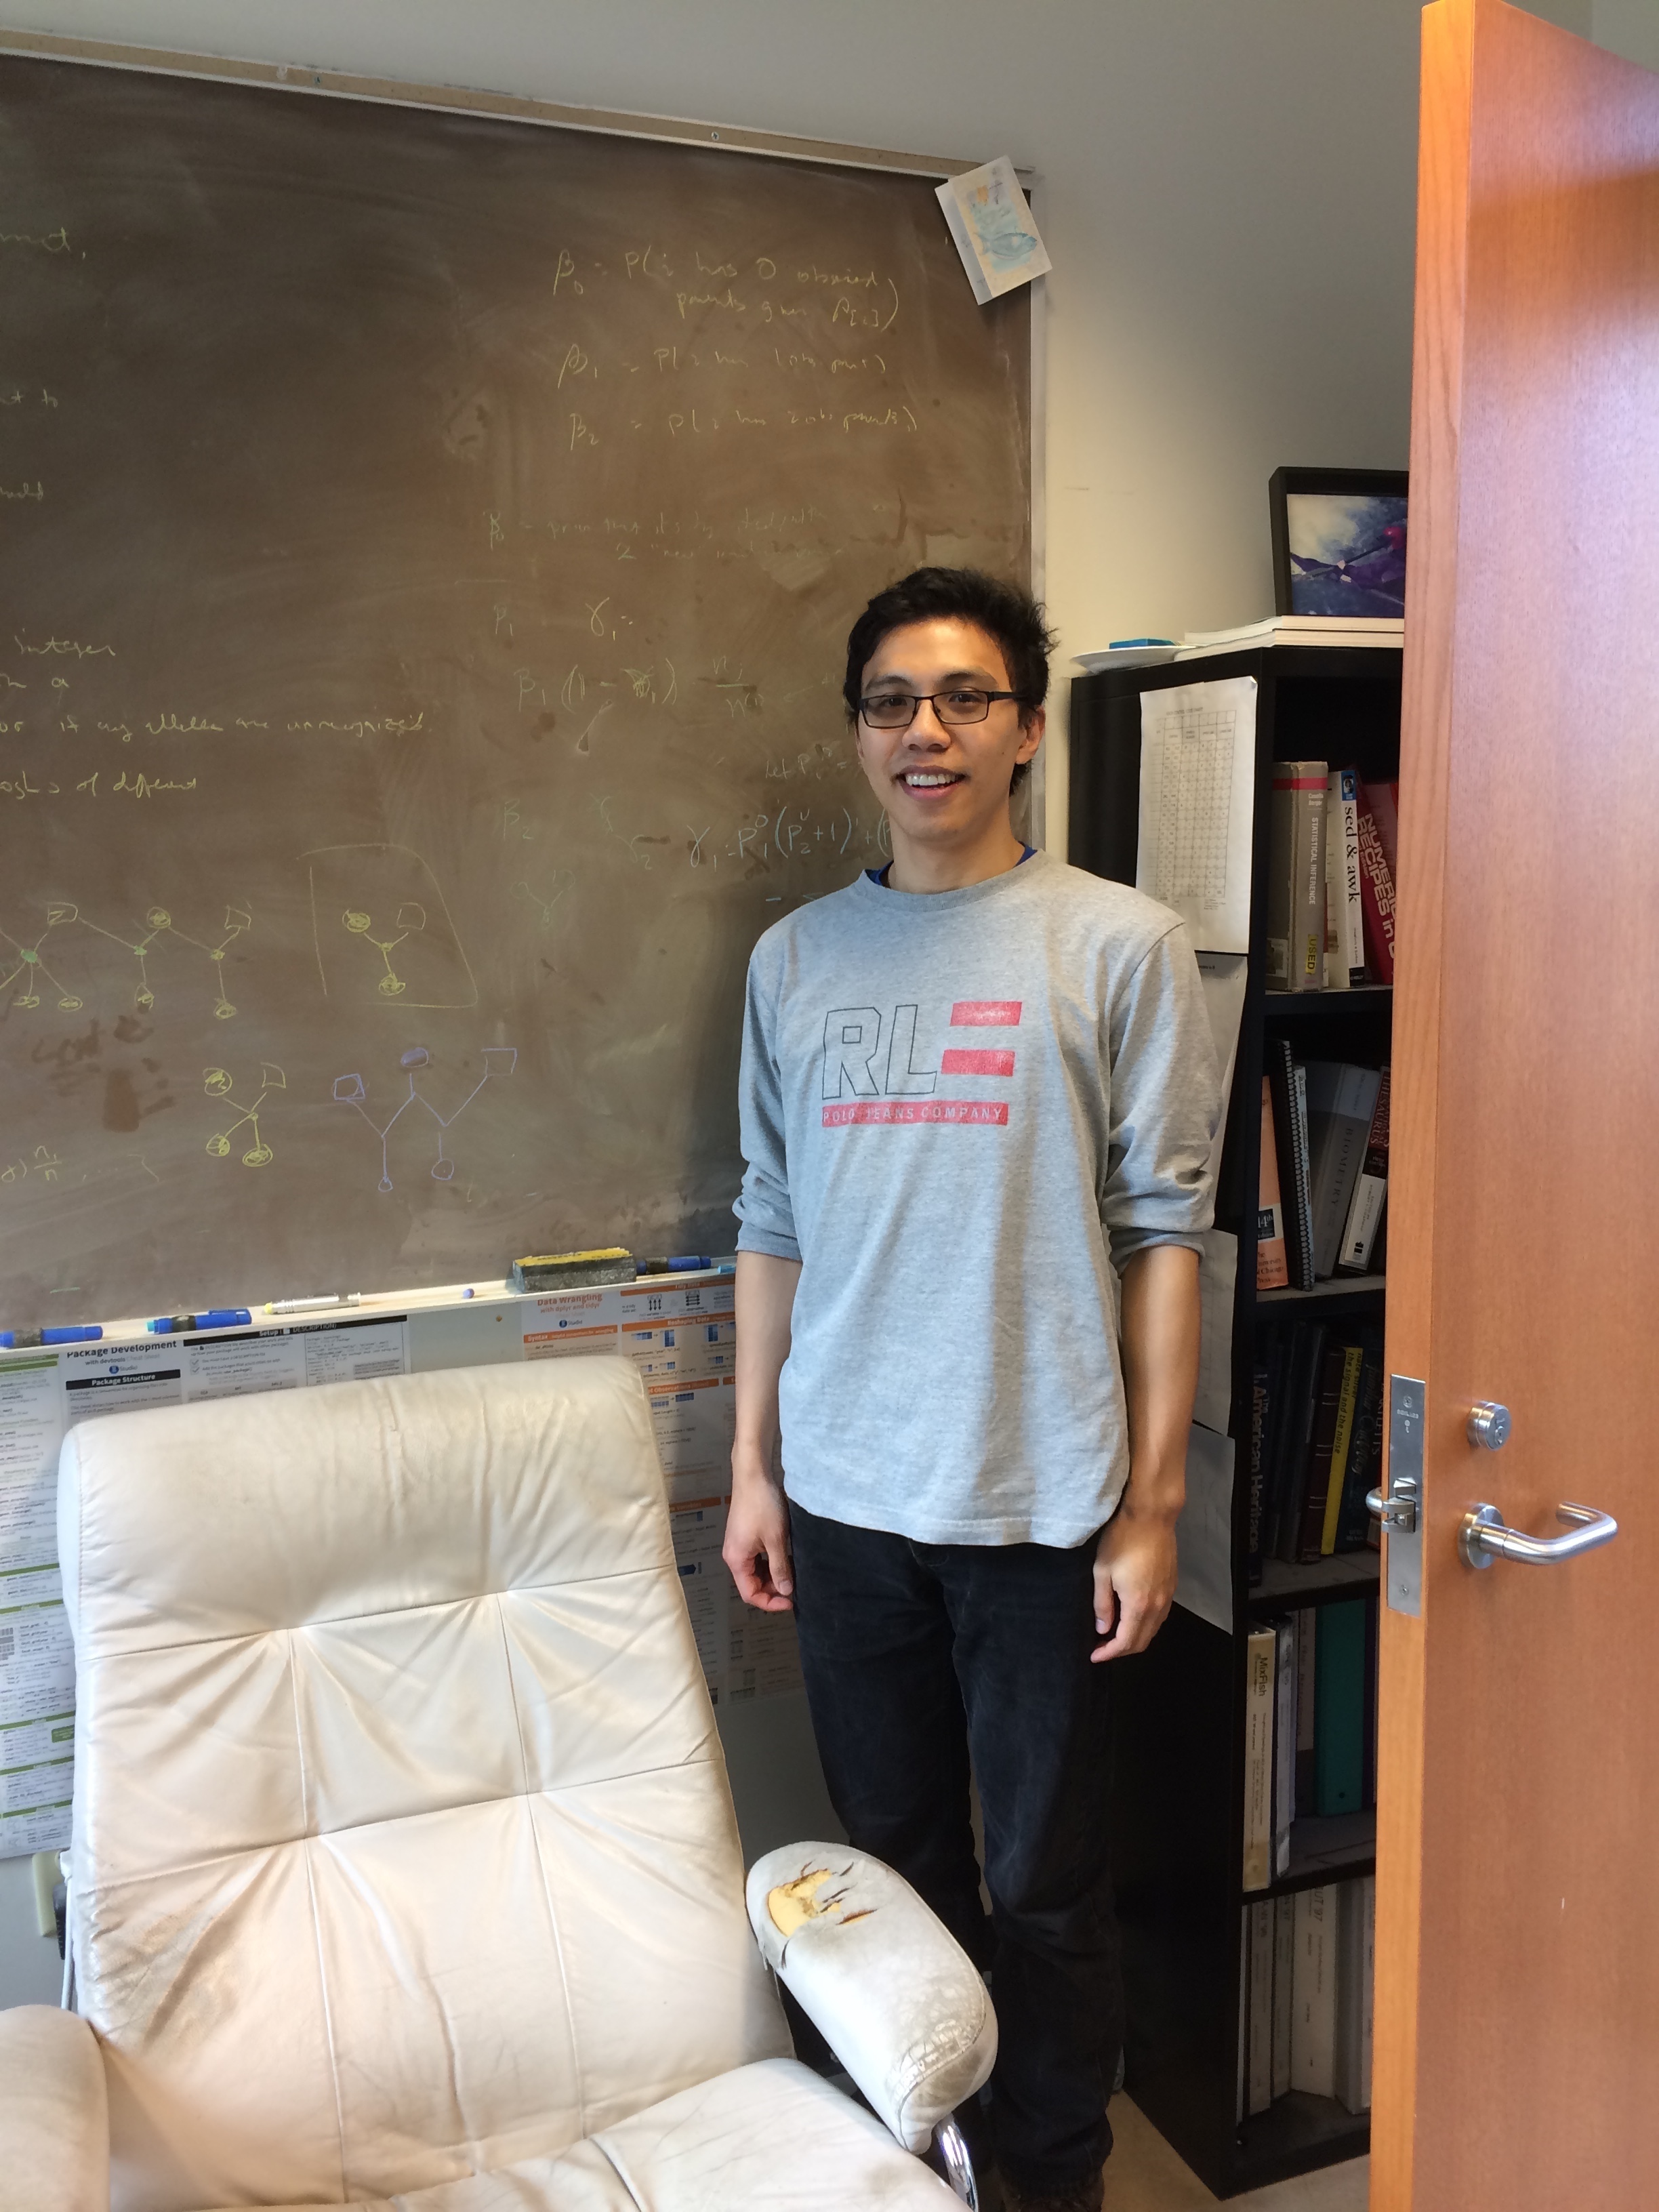
\includegraphics[width = 0.8\textwidth]{figs/thomas.jpg}
\end{column}
\end{columns}

\end{frame}

\newpage
\mbox{}
\vspace*{2em}
\mbox{}
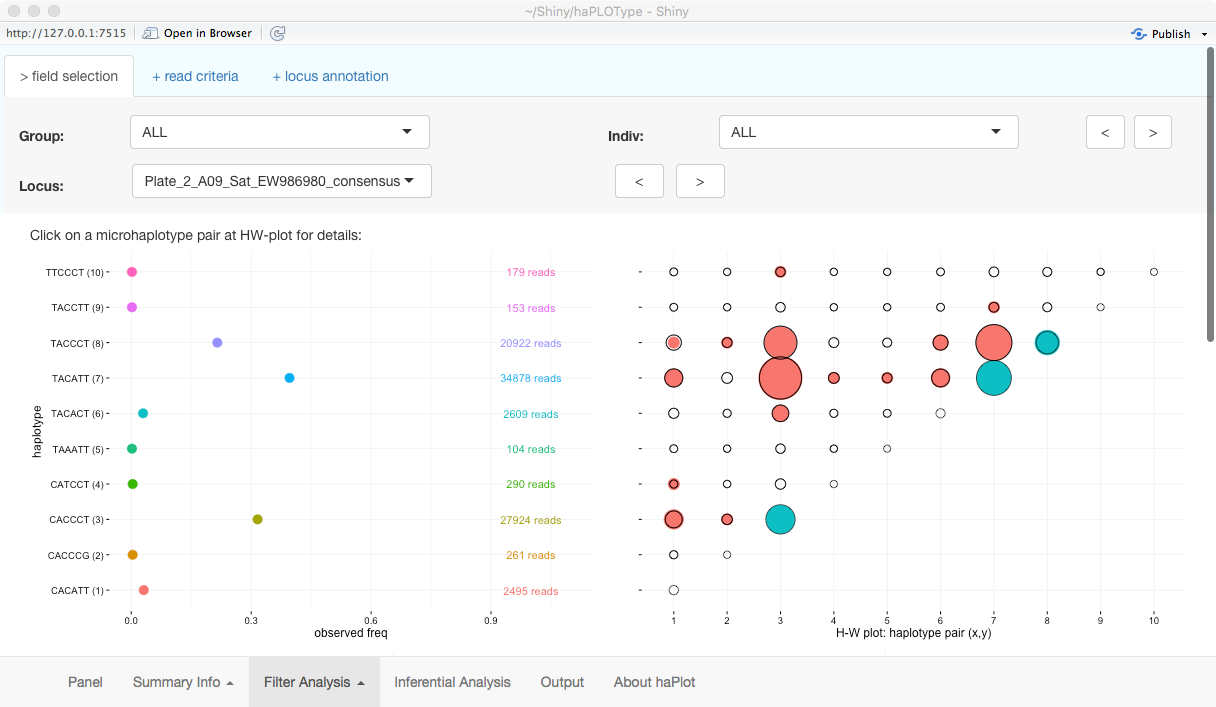
\includegraphics[width=\textwidth]{figs/haplot2.png}



\begin{frame}{How Well Does It Work? --- Roadmap}

\begin{itemize}
\item Works on multiple species?  Yes! grad student Hayley Nuetzel just completed species ID work with 24 species.  With very little missing data, and highly accurate species assignments.
\item Haplotype Diversity in Kelp Rockfish
\item Genotype Quality / Accuracy:
\begin{itemize}
\item Sequence Read Depths
\item Distortions from Hardy-Weinberg Proportions
\item Regenotype Discordance Rate
\end{itemize}
\item Preliminary Results from Relationship Inference
\end{itemize}
\end{frame}



\begin{frame}{Allele/Haplotype Diversity}
\framesubtitle{In 96 Loci in Kelp Rockfish: 1039 Unique Alleles in total!}
\begin{center}
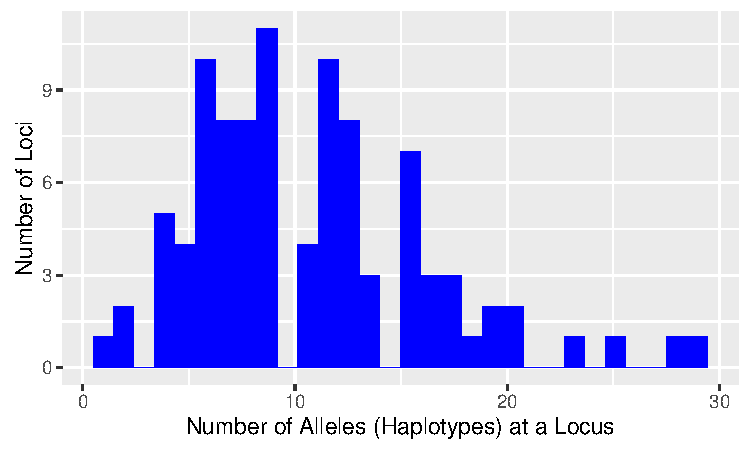
\includegraphics[width = 0.8\textwidth]{figs/alle-count-histo.pdf}
\end{center}
\end{frame}




\begin{frame}{Read Depths For Calling Alleles}
\framesubtitle{Much higher than low-coverage genome work}

Across $\approx$15,000 individuals and at all 96 loci, called-allele read depths 
were as follows:

\begin{center}
\begin{tabular}{lrrr}
Read Depth Bin  &  n  &  Percentage  &  Cumulative\\ \hline
(0,10]  &  3859  &  0.2  &  0.2\\
(10,20]  &  20509  &  1.1  &  1.3\\
(20,30]  &  34903  &  1.9  &  3.2\\
(30,40]  &  44896  &  2.4  &  5.6\\
(40,50]  &  50964  &  2.8  &  8.4\\
(50,75]  &  138593  &  7.5  &  15.9\\
(75,100]  &  136191  &  7.4  &  23.3\\
(100,250]  &  637913  &  34.5  &  57.8\\
(250,500]  &  484226  &  26.2  &  83.9\\
(500,1e+03]  &  234141  &  12.7  &  96.6\\
(1e+03,1e+06]  &  62604  &  3.4  &  100.0\\
\end{tabular}
\end{center}
\end{frame}





\begin{frame}{Expected-vs-observed rate of homozygotes\ldots}
\framesubtitle{Allele-specific Homozygosities from $\approx$ 6,000 kelp rockfish}
Green = 10 loci with null alleles.  Orange = 86 remaining loci
\begin{center}
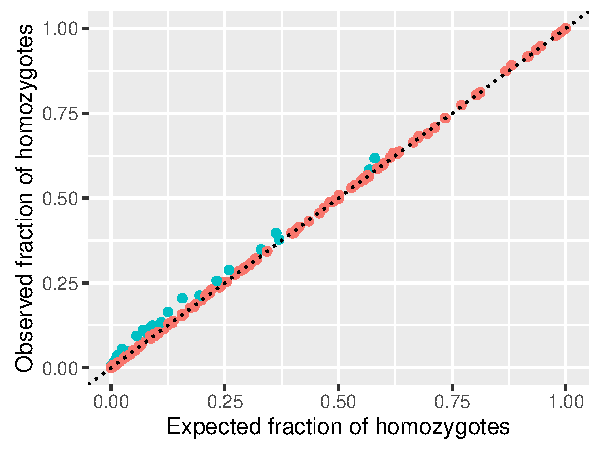
\includegraphics[width=.7\textwidth]{./figs/microhap_homozyg.pdf}
\end{center}
$\bullet$ Null alleles can be treated systematically.\\
$\bullet$ From 75 kelp rockfish genotyped twice, the per-locus discordance rate was 3/1000.
\end{frame}














\begin{frame}{Log-likelihood ratio distribution}
\framesubtitle{For Parent-offspring and full-sib pairs vs Unrelated}
\begin{center}
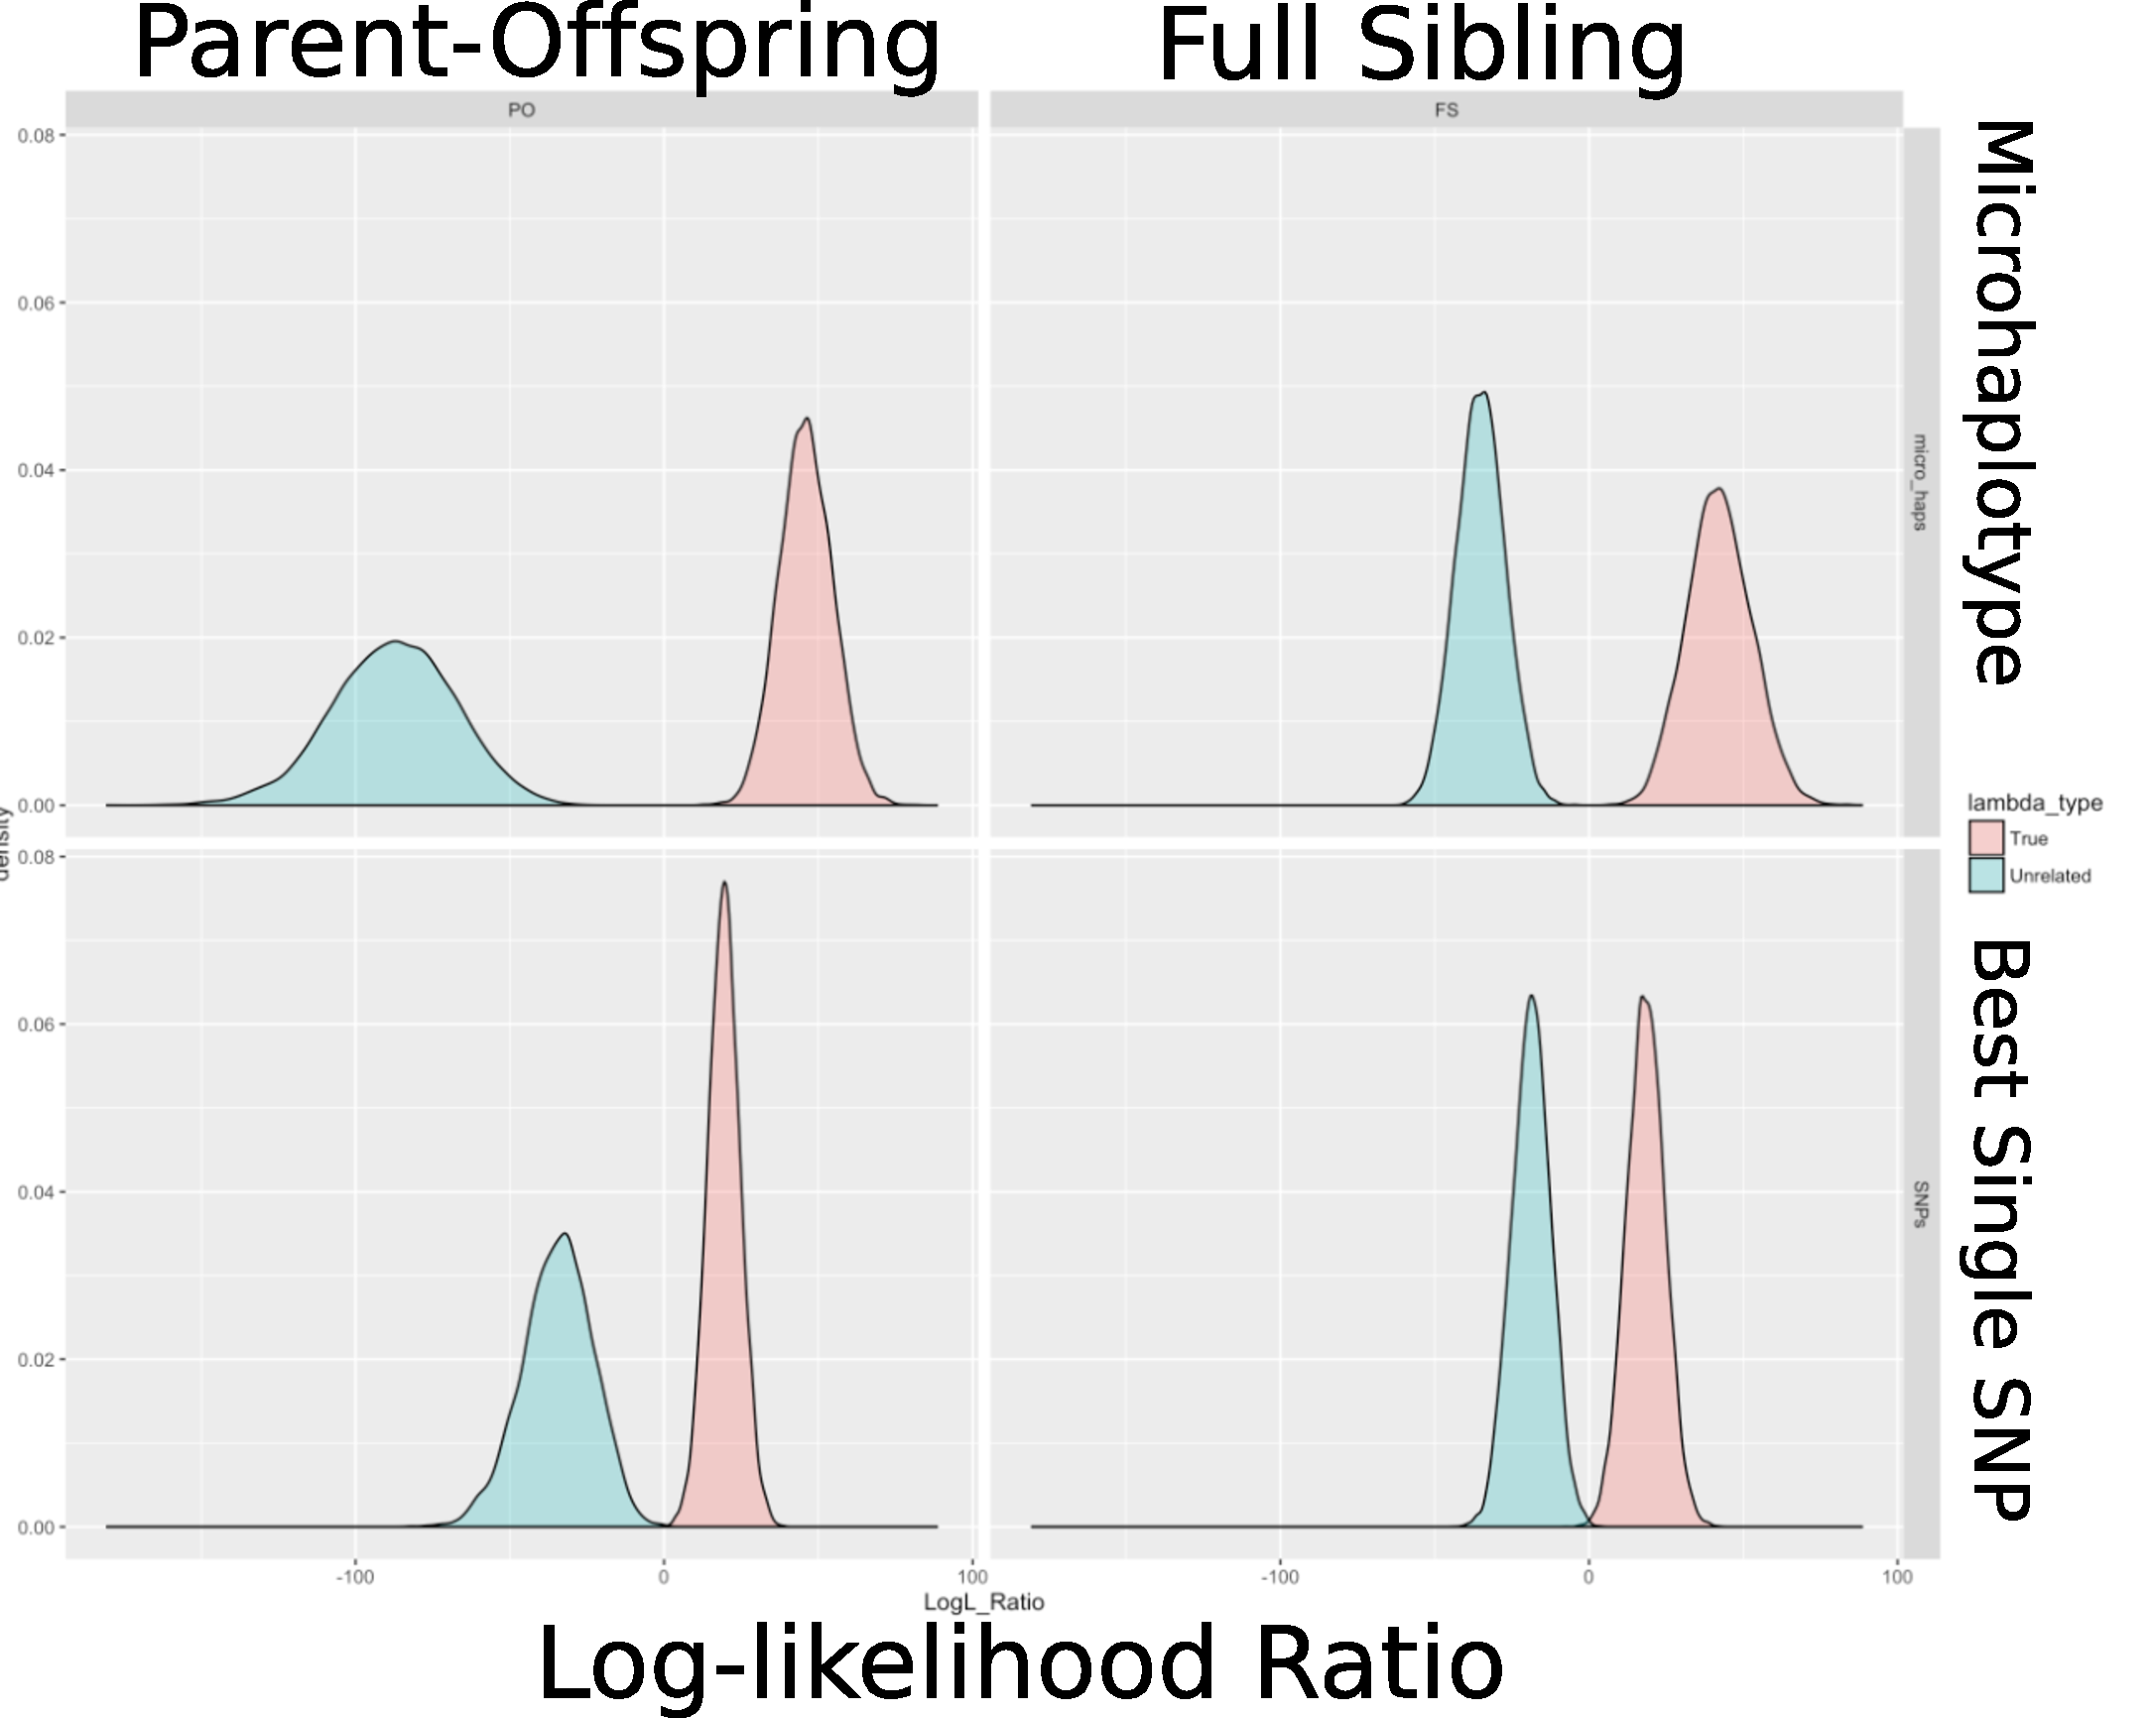
\includegraphics[width = 0.84\textwidth]{mhap_figs/loglrats.pdf}
\end{center}

\end{frame}













\begin{frame}{Log-likelihood ratio distribution}
\framesubtitle{False Positive Rates for Unrelated individuals at False Negative Rate = 1\%}
\begin{center}
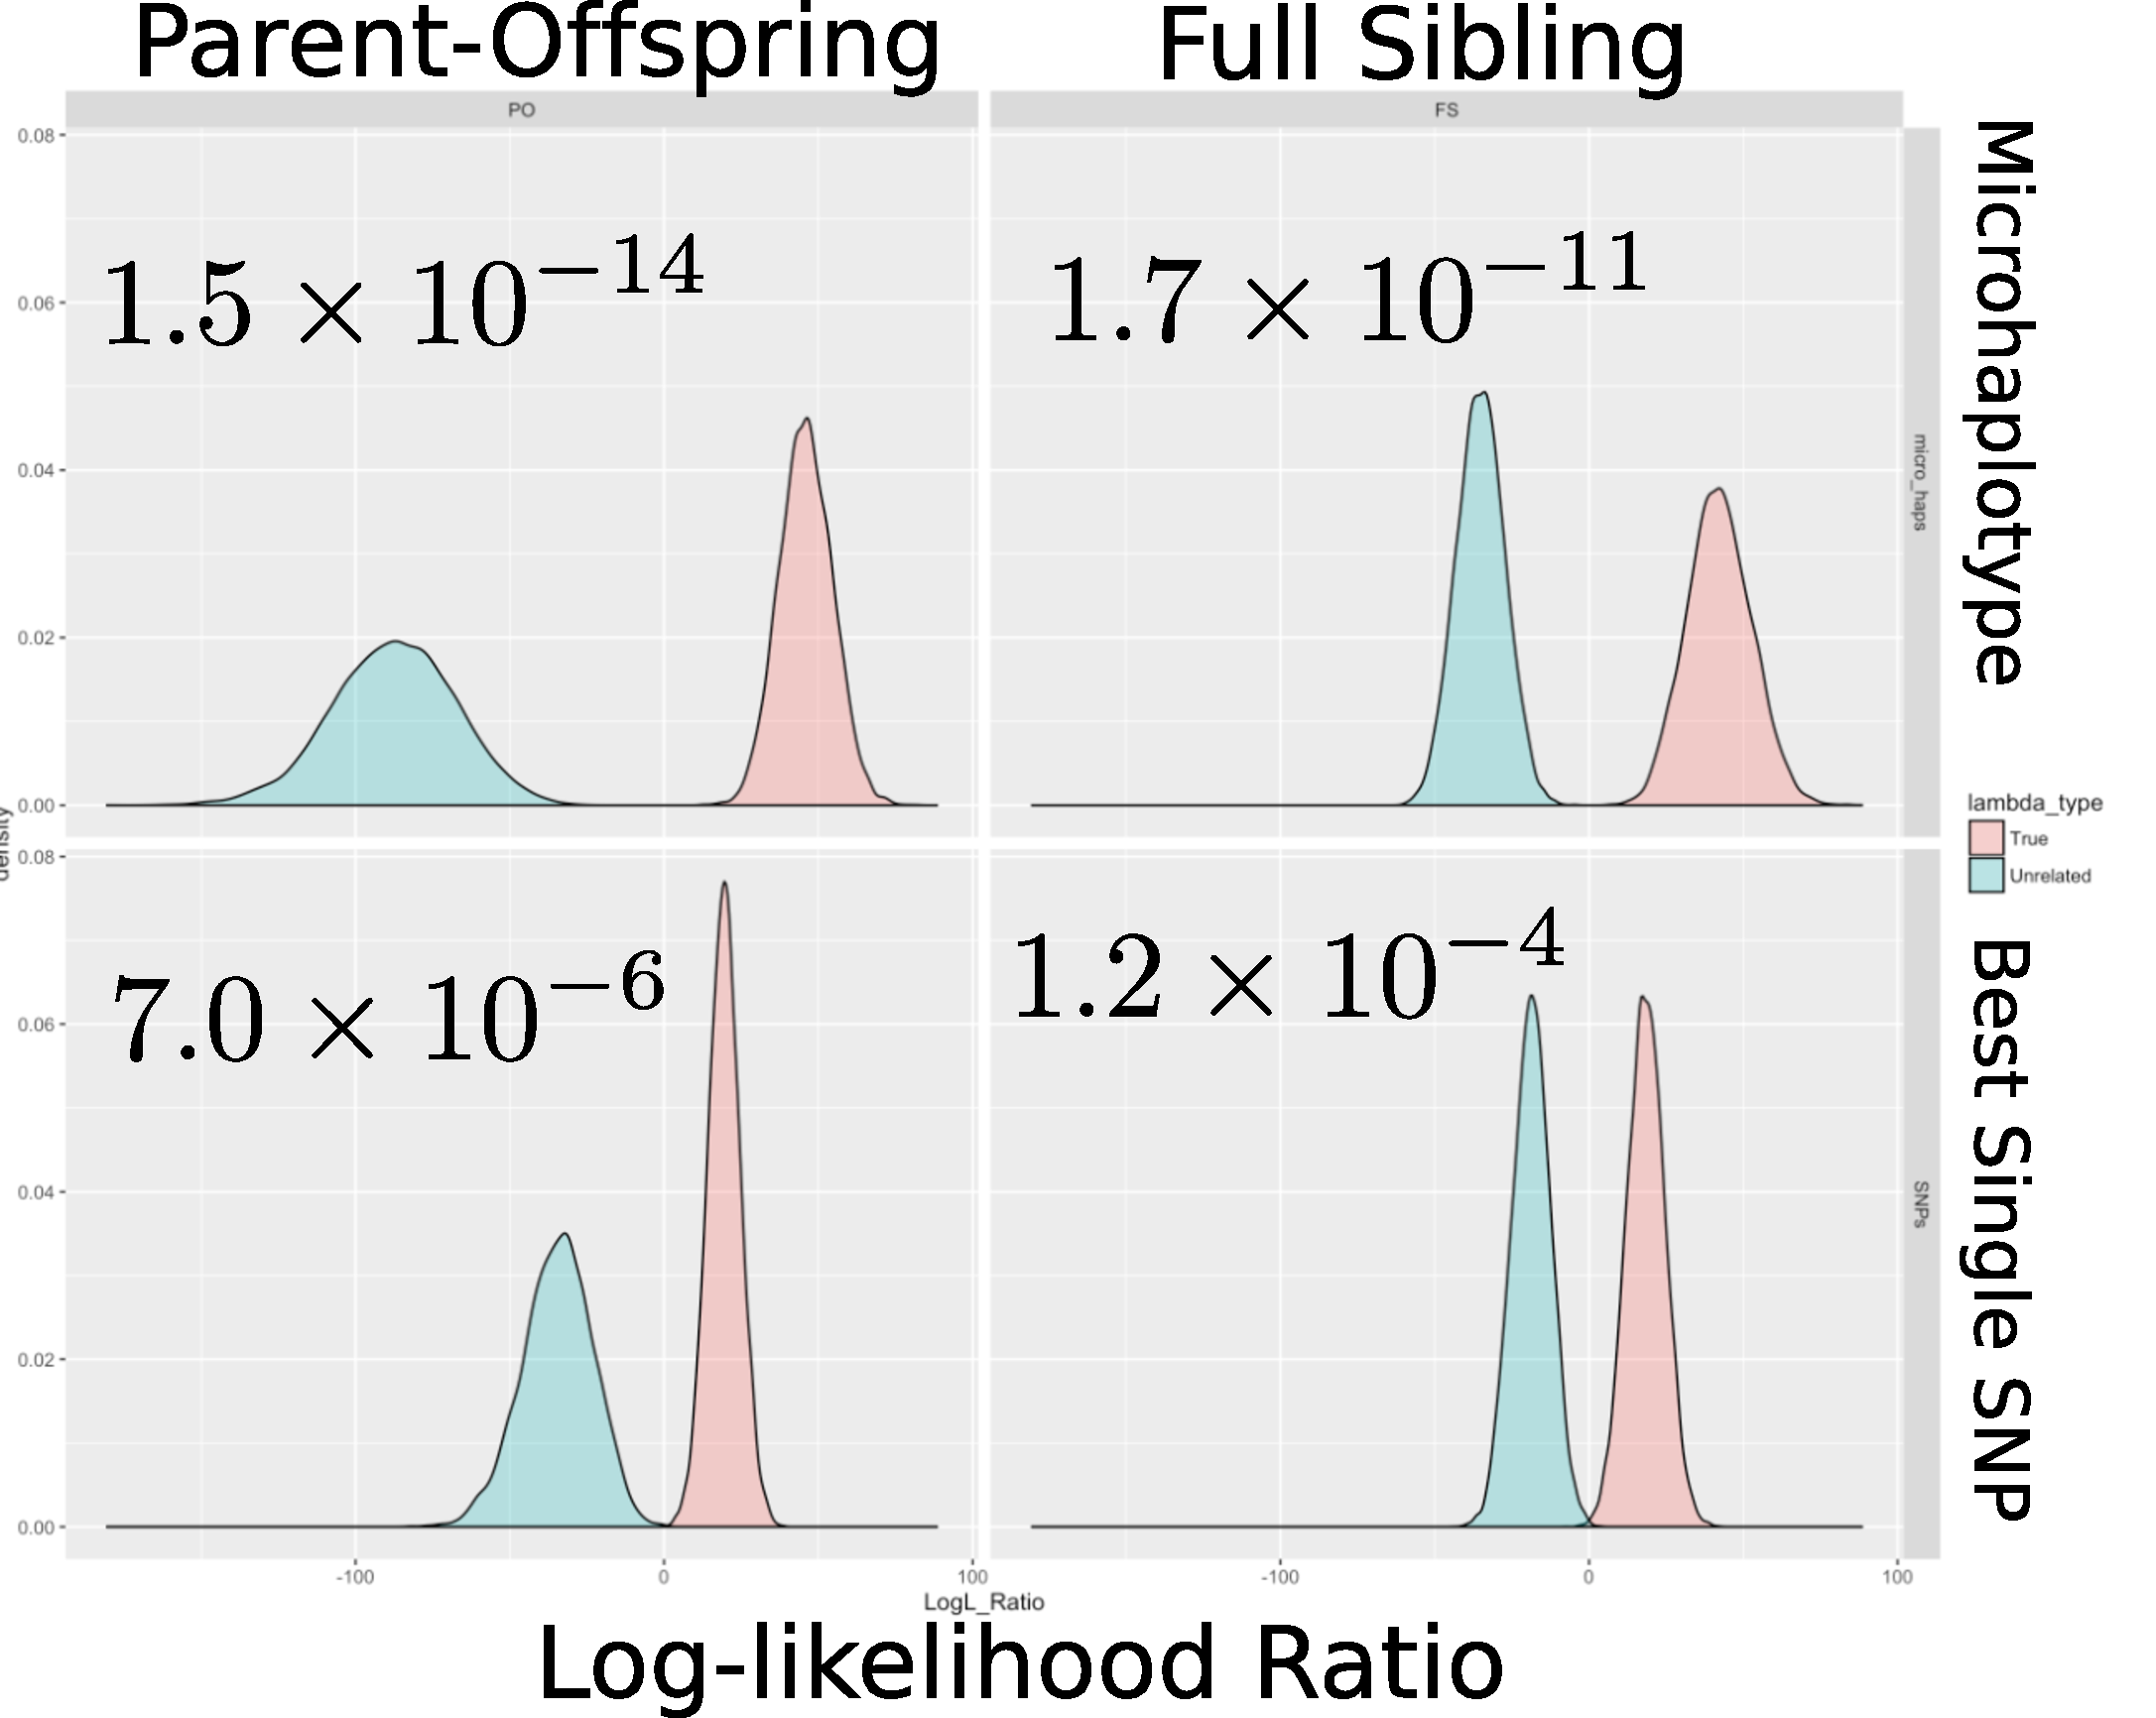
\includegraphics[width = 0.84\textwidth]{mhap_figs/loglrats-FPR.pdf}
\end{center}

\end{frame}












\begin{frame}{Outstanding for Relationship Inference}
\begin{itemize}
\item A false positive rate of $1.5 \times 10^{-14}$ means you could compare 1 million candidate parents to 1 million unrelated candidate offspring and not expect any errors.
\item Using just a single SNP from each locus you would expect 7 errors when comparing 1,000 candidate parents to 1,000 unrelated candidate offspring.
\item Genotyping costs dropping toward $<$\textsterling 5 per sample.
\item Very exciting for ``close-kin mark-recapture''\\
{\em Statistical Science}~31:259--274. (2016)
\end{itemize}
\begin{center}

\includegraphics[width = 0.7\textwidth]{mhap_figs/ckmr-header.png}
\end{center}
\end{frame}




\begin{frame}{The Prospects for Half-Sibling Identification}
\begin{center}
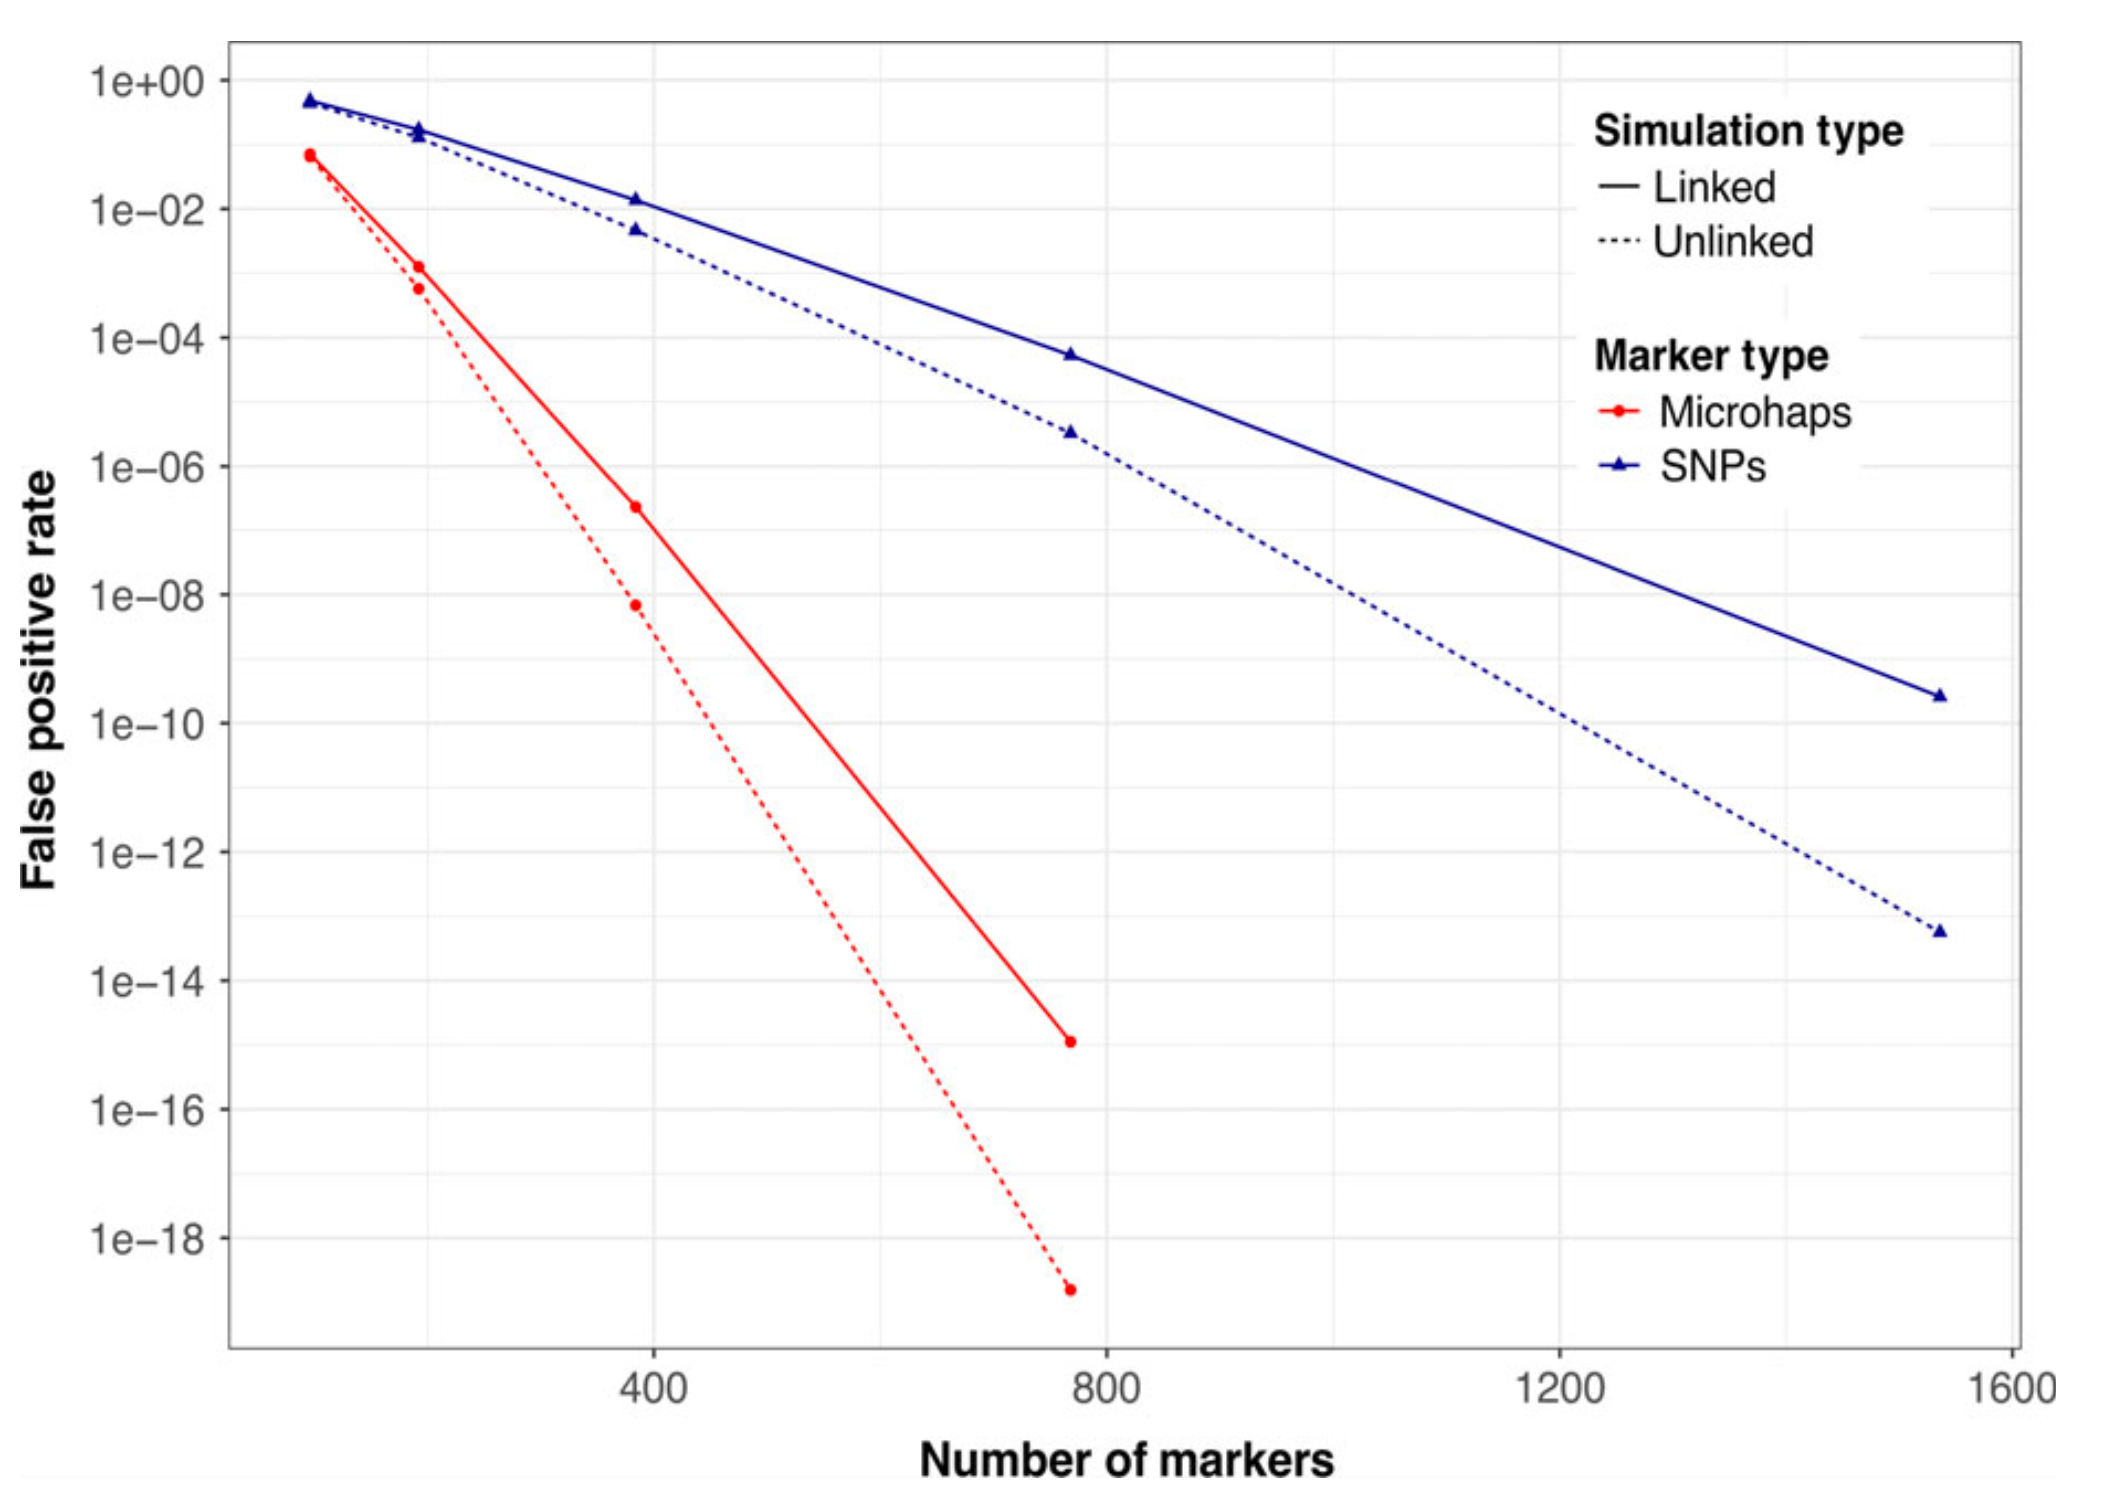
\includegraphics[width = 0.8\textwidth]{../figures/linked-power.png}
\end{center}
\end{frame}





\begin{frame}{{\tt microhaplot} overview of workflow}
\framesubtitle{R package by Thomas Ng}

\begin{itemize}
\item PCR amplify amplicons, or otherwise select a small portion of the genome (100 to 5000 chunks, each about 150 bp long) and sequence those
regions in many barcoded individuals.
\item Align those reads to a ``genome,'' (which might even just be the sequences that you expect from the regions that you have amplified.)
\item Call SNPs in those regions.  Put those variant calls in a VCF file.
\item Filter those variants into ones that you are confident about and create what we can call
our ``input VCF'' file.  This is the file that tells {\tt microhaplot} at which positions it should look to
find and record variants.  

\end{itemize}
\end{frame}


\begin{frame}{}
\begin{itemize}
\item Feed the input VCF and the SAM files (alignment files) into {\tt microhaplot}.  It then parses the SAMs and records the bases at each position that is named in the input VCF.  Nucleotides that occur together
on the same read are the ``microhaplotypes.'' 
\begin{itemize}
 \item Note: there is no statistical phasing going on here.
 \item The tricky part in this is parsing the CIGAR string to figure out which positions in the reads
 correspond to the desired positions in the reference.
\end{itemize}

\item Visualize, filter, interpret, and output data while using {\tt microhaplot}
\begin{itemize}
\item This is what we will do together today (we won't work so much with the previous bioinformatics steps,
but, rather, we just want to familiarize people with the {\tt microhaplot} interface.  
\item Talk to me or Thomas about getting your own data into {\tt microhaplot}.
\end{itemize}

\item Goto: {\tt https://github.com/ngthomas/microhaplot}

\end{itemize}


\end{frame}


\end{document}



